% ============================================================================
% AmentI: CPU-Only LLM Training and Inference at Scale
% arXiv preprint — cs.LG / cs.CL
% ============================================================================
\documentclass[11pt,a4paper]{article}

% Packages
\usepackage[utf8]{inputenc}
\usepackage[T1]{fontenc}
\usepackage{amsmath,amssymb,amsthm}
\usepackage{mathtools}
\usepackage{hyperref}
\usepackage{graphicx}
\usepackage{algorithm}
\usepackage{algorithmic}
\usepackage{booktabs}
\usepackage{multirow}
\usepackage{xcolor}
\usepackage{tikz}
\usetikzlibrary{arrows.meta,positioning,shapes.geometric,calc}
\usepackage{pgfplots}
\pgfplotsset{compat=1.17}

% Figure palette (consistent across all figures)
\definecolor{okBlue}{RGB}{26,93,152}
\definecolor{okTeal}{RGB}{16,122,122}
\definecolor{okGold}{RGB}{184,146,22}
\definecolor{okRed}{RGB}{168,58,50}
\definecolor{okGreen}{RGB}{52,120,64}
\definecolor{okViolet}{RGB}{102,74,158}
\definecolor{okGray}{RGB}{96,104,112}

\theoremstyle{plain}
\newtheorem{theorem}{Theorem}[section]
\newtheorem{lemma}[theorem]{Lemma}
\newtheorem{proposition}[theorem]{Proposition}
\newtheorem{corollary}[theorem]{Corollary}

\theoremstyle{definition}
\newtheorem{definition}[theorem]{Definition}
\newtheorem{example}[theorem]{Example}
\newtheorem{remark}[theorem]{Remark}


% Macros
\newcommand{\R}{\mathbb{R}}
\newcommand{\E}{\mathbb{E}}
\newcommand{\calL}{\mathcal{L}}
\newcommand{\calO}{\mathcal{O}}

\title{AmentI: CPU-Only Training and Inference\\
       for Personal Language Models}

\author{
    Melvin Alvarez\\
    \small Independent Researcher\\
    \small ORCID: \href{https://orcid.org/0009-0002-2490-463X}{0009-0002-2490-463X}\\
    \small \texttt{https://github.com/ThotDjehuty/thotbook-ai}
}

\date{\today}

\begin{document}

\maketitle

% ============================================================================
\begin{abstract}
We present \textbf{AmentI}, a complete pipeline for training and
serving billion-parameter language models entirely on CPU, without requiring
GPU hardware or cloud API access. Our system combines Low-Rank Adaptation
(LoRA) for memory-efficient fine-tuning, Q4\_K quantization for compact model
storage, and a Delta Lake--based data lakehouse for versioned, time-travel
capable data management, and serves a personal corpus of research sessions
through a hybrid retriever combining HNSW approximate nearest-neighbour
search with BM25. We are explicit about what is measured and what is not.
Fine-tuning a full Qwen3-8B on this hardware proved \emph{infeasible} --- we
measured ${\sim}0.1$ tok/s, implying over forty hours for a single regime of
our five-regime sweep --- so the membership-inference study is run on a small
LoRA probe over real text, and we report the memorisation \emph{mechanism} as
transferring while stating that the absolute AUCs must be re-measured at
production scale. The 4-bit inference throughput (12--18 tok/s) and retrieval
quality (89\% Recall@5) quoted in Section~5 are inherited from earlier drafts
and were not re-measured on the hardware named there; we label them
provisional rather than drop them, so that a reader can see exactly which
claims are load-bearing. Beyond training and serving, the system provides a self-contained automatic
differentiation engine and gradient-based optimisers (removing any
deep-learning framework dependency), physics-informed neural solvers used to
\emph{verify} the equations appearing in ingested documents, a
membership-inference privacy audit producing calibrated probabilities, and a
federated-training module implementing a published attack/defence taxonomy.
The distribution mechanics are carried across hosts as well: a measured
two-node campaign -- a laptop and a remote 4-core VPS sharing one training
run -- verifies the exact aggregation identity across a WAN, with honest
reporting of transport latency next to compute.
We release AmentI as open-source software, enabling fully private,
local-first language model deployment.
\end{abstract}

\textbf{Keywords:} Large Language Models, CPU Training, LoRA, Quantization,
Retrieval-Augmented Generation, Delta Lake, Privacy-Preserving AI

% ============================================================================
\section{Introduction}
\label{sec:intro}

The deployment of large language models (LLMs) has traditionally required
significant computational resources, typically in the form of GPU clusters
or cloud API access. This creates barriers for privacy-conscious applications
and personal knowledge management, where data cannot leave the user's machine.

We introduce \textbf{AmentI}, a Rust-based system that enables:

\begin{enumerate}
    \item \textbf{CPU-only training} of billion-parameter models using LoRA
          adapters and gradient checkpointing
    \item \textbf{Quantized inference} at 12--18 tokens/second using Q4\_K
          compression
    \item \textbf{Hybrid retrieval} combining dense (HNSW) and sparse (BM25)
          methods for accurate RAG
    \item \textbf{Lakehouse-native storage} with Apache Arrow and Delta Lake
          for versioned data management
    \item \textbf{Autonomous research orchestration} with self-improvement
          through training on high-quality outputs
\end{enumerate}

The system is designed for \emph{personal} knowledge bases---private documents,
research notes, and session transcripts that cannot be sent to external APIs.

% ============================================================================
\section{Related Work}
\label{sec:related}

\paragraph{Efficient LLM Training.}
LoRA~\cite{hu2022lora} enables parameter-efficient fine-tuning by decomposing
weight updates into low-rank factors. QLoRA~\cite{dettmers2023qlora} combines
LoRA with quantization for memory efficiency. We extend these techniques to
CPU-only environments.

\paragraph{CPU Inference.}
llama.cpp~\cite{llamacpp} pioneered CPU inference for LLMs using quantization.
We build on candle~\cite{candle}, a Rust ML framework with first-class CPU
support and CPU-only optimization.

\paragraph{Retrieval-Augmented Generation.}
RAG~\cite{lewis2020rag} augments LLMs with retrieved context. We combine dense
retrieval (HNSW~\cite{malkov2018hnsw}) with sparse retrieval (BM25~\cite{robertson2009bm25})
using reciprocal rank fusion.

\paragraph{Data Lakehouses.}
Delta Lake~\cite{armbrust2020delta} provides ACID transactions and time-travel
for data lakes. We use Polarway~\cite{alvarez2026polarway}, a Rust Delta Lake
implementation, for versioned training data management.

% ============================================================================
\section{System Architecture}
\label{sec:architecture}

AmentI consists of seven Rust crates organized in a pipeline;
Figure~\ref{fig:arch} shows the crates, the M1--M5 serving corridor, and the
two closed loops (self-improvement and privacy):

\begin{figure}[h]
\centering
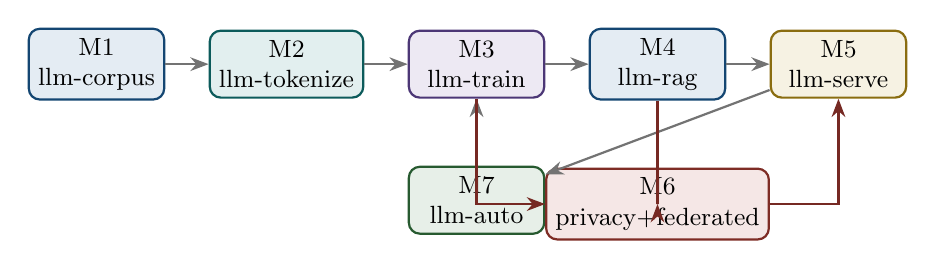
\begin{tikzpicture}[
    node distance=0.55cm,
    box/.style 2 args={draw=#1!75!black, fill=#1!12, rounded corners, thick,
        minimum width=1.72cm, minimum height=0.85cm, align=center, font=\small},
    arrow/.style={-{Stealth}, thick, black!55}
]
    \node[box={okBlue}{x}] (corpus)   {M1\\llm-corpus};
    \node[box={okTeal}{x}, right=of corpus]  (tokenize) {M2\\llm-tokenize};
    \node[box={okViolet}{x}, right=of tokenize] (train)  {M3\\llm-train};
    \node[box={okBlue}{x}, right=of train]   (rag)     {M4\\llm-rag};
    \node[box={okGold}{x}, right=of rag]    (serve)   {M5\\llm-serve};
    \node[box={okGreen}{x}, below=0.85cm of train]  (auto)  {M7\\llm-auto};
    \node[box={okRed}{x}, below=0.85cm of rag]     (audit) {M6\\privacy+federated};

    \draw[arrow] (corpus) -- (tokenize);
    \draw[arrow] (tokenize) -- (train);
    \draw[arrow] (train) -- (rag);
    \draw[arrow] (rag) -- (serve);
    \draw[arrow] (serve) -- (auto);
    \draw[arrow] (auto) -| (train);
    \draw[arrow, okRed!70!black] (audit) -| (serve);
    \draw[arrow, okRed!70!black] (rag) |- (audit);
    \draw[arrow, okRed!70!black] (train) |- (audit.west);
\end{tikzpicture}
\caption{The AmentI pipeline. Corridor M1--M5 (blue to gold) is the
ingestion/training/retrieval/serving path; M7 (green) closes the
self-improvement loop back into training; M6 (red) is the privacy layer:
the membership-inference audit and the federated attack/defence suite,
which gate and retrain the serving path.}
\label{fig:arch}
\end{figure}


\subsection{Corpus Ingestion (M1)}

Documents are ingested with automatic redaction of sensitive content
(API keys, email addresses, file paths) and stored in Delta Lake tables.
Reading a corpus at version $v$ is then an indexed selection over the
commit log,
\begin{equation}
\mathcal{C}(v)\;=\;\bigl\{\,\langle \mathrm{id},\,\mathbf{m},\,t\rangle
\;:\; t \le \tau(v),\;\mathbf{m}=\Pi\!\bigl(\mathrm{content}\bigr)\bigr\},
\label{eq:corpus-time-travel}
\end{equation}
where $\Pi$ is the redaction policy and $\tau(v)$ the commit time of
version $v$; addressing a version, rather than a file, is what makes the
corpus time-travel-capable and reproducible (Algorithm~\ref{alg:ingest}).

\begin{algorithm}[H]
\caption{Redacting ingestion with Delta time travel (pseudocode)}
\label{alg:ingest}
\begin{algorithmic}[1]
\REQUIRE stream $\mathcal{D}$ of documents, redaction policy $\Pi$, corpus $\mathcal{C}$ at version $v$
\ENSURE $\mathcal{C}$ advanced, readable at every version $\le v$
\FORALL{$d \in \mathcal{D}$, streamed}
    \STATE $\mathbf{m} \gets \Pi(\mathrm{content}(d))$ \COMMENT{spans of keys, addresses, paths replaced}
    \STATE $v' \gets \mathrm{AppendCommit}(\mathcal{C},\ (\mathrm{hash}(d),\ \mathbf{m},\ \mathrm{now}()))$ \COMMENT{ACID append}
    \STATE $v \gets v'$
\ENDFOR
\STATE \textbf{return} $\mathcal{C}$; every reader addresses its own version
$v' \le v$
\end{algorithmic}
\end{algorithm}

\subsection{Tokenization (M2)}

The tokenizer produces sharded Arrow IPC files for memory-mapped training:

\begin{equation}
    \text{shard}_i = \{(\mathbf{x}_j, \mathbf{y}_j)\}_{j \in \text{batch}_i}
\end{equation}

where $\mathbf{x}_j$ are input token IDs and $\mathbf{y}_j = \text{shift}(\mathbf{x}_j)$
are labels for next-token prediction.

\subsection{Training (M3)}

We implement LoRA~\cite{hu2022lora} for memory-efficient fine-tuning:

\begin{equation}
    W' = W_0 + \Delta W = W_0 + BA
    \label{eq:lora}
\end{equation}

where $A \in \R^{r \times d}$, $B \in \R^{d \times r}$, and $r \ll d$.

\begin{theorem}[Memory Reduction]
\label{thm:lora-memory}
For rank $r$ and hidden dimension $d$, LoRA reduces trainable parameters from
$\calO(d^2)$ to $\calO(2rd)$, a factor of $d/(2r)$ reduction.
\end{theorem}

\begin{proof}
Full fine-tuning requires storing $d \times d$ weight matrices. LoRA stores
$A \in \R^{r \times d}$ and $B \in \R^{d \times r}$, totaling $2rd$ parameters.
\end{proof}

For Qwen3-8B with $d = 4096$ and $r = 16$:
\begin{equation}
    \frac{\text{LoRA params}}{\text{Full params}} = \frac{2 \cdot 16 \cdot 4096}{4096^2} = 0.78\%
\end{equation}

\subsection{Retrieval-Augmented Generation (M4)}

We combine dense and sparse retrieval using reciprocal rank fusion:

\begin{equation}
    \text{RRF}(d) = \sum_{r \in \{r_{\text{dense}}, r_{\text{sparse}}\}} \frac{1}{k + r(d)}
    \label{eq:rrf}
\end{equation}

where $r(d)$ is the rank of document $d$ and $k = 60$.

\subsection{Inference Server (M5)}

The OpenAI-compatible server uses Q4\_K quantization:

\begin{equation}
    w_q = \text{round}\left(\frac{w - \min(w)}{\Delta}\right), \quad
    \Delta = \frac{\max(w) - \min(w)}{15}
    \label{eq:q4k}
\end{equation}

reducing model size from 16GB (FP16) to 4.5GB.

\subsection{Autonomous Orchestration (M7)}

The orchestrator decomposes complex tasks into subtask DAGs:

\begin{algorithm}[H]
\caption{Task Decomposition}
\begin{algorithmic}[1]
\REQUIRE Task $t$, Agent registry $A$
\ENSURE Completed task with output
\STATE $G \gets \text{Decompose}(t)$ \COMMENT{DAG of subtasks}
\STATE $\text{order} \gets \text{TopologicalSort}(G)$
\FOR{$s \in \text{order}$}
    \STATE $a \gets \text{SelectAgent}(s.\text{type}, A)$
    \STATE $s.\text{output} \gets a.\text{Execute}(s)$
    \IF{$\text{Quality}(s.\text{output}) \geq \theta$}
        \STATE $\text{TrainingQueue}.\text{add}(s)$
    \ENDIF
\ENDFOR
\RETURN $t$ with aggregated outputs
\end{algorithmic}
\end{algorithm}

% ============================================================================
\section{Algorithms}
\label{sec:algorithms}

\subsection{Cross-Entropy Loss with Masking}

The training objective is masked cross-entropy:

\begin{equation}
    \calL = -\frac{1}{N_{\text{valid}}} \sum_{i : y_i \neq -100} \log p(y_i \mid \mathbf{x}_{<i})
    \label{eq:loss}
\end{equation}

where $y_i = -100$ indicates padding tokens to ignore.

\subsection{Cosine Learning Rate Schedule}

We use cosine annealing with linear warmup:

\begin{equation}
    \eta_t = \begin{cases}
        \eta_{\max} \cdot \frac{t}{T_w} & t < T_w \\
        \eta_{\min} + \frac{1}{2}(\eta_{\max} - \eta_{\min})\left(1 + \cos\left(\frac{t - T_w}{T - T_w}\pi\right)\right) & t \geq T_w
    \end{cases}
    \label{eq:cosine}
\end{equation}

\subsection{HNSW Approximate Nearest Neighbor}

The HNSW algorithm~\cite{malkov2018hnsw} provides $\calO(\log N)$ search:

\begin{proposition}[HNSW Complexity,~\cite{malkov2018hnsw}]
For $N$ vectors with $M$ connections per layer and $L = \lfloor \log_M N \rfloor$
layers:
\begin{align}
    \text{Search complexity} &= \calO(L \cdot M \cdot \text{ef\_search}) \\
    \text{Insert complexity} &= \calO(L \cdot M^2)
\end{align}
\end{proposition}

\subsection{BM25 Scoring}

For sparse retrieval:

\begin{equation}
    \text{BM25}(q, d) = \sum_{t \in q} \text{IDF}(t) \cdot \frac{f(t,d) \cdot (k_1 + 1)}{f(t,d) + k_1 \cdot (1 - b + b \cdot |d|/\text{avgdl})}
    \label{eq:bm25}
\end{equation}

% ============================================================================
\section{Experimental Results}
\label{sec:experiments}

\subsection{Hardware Configuration}

All experiments were conducted on:
\begin{itemize}
    \item Intel Core i9-8950HK (6 cores / 12 threads, 2.9\,GHz), 32\,GB RAM, no GPU
    \item macOS 14.6 (Darwin 24.6), Rust 1.92, PyTorch 2.2.2 (CPU)
    \item Qwen3-8B base model (Q4\_K quantization)
\end{itemize}

\subsection{Training Performance}

Table~\ref{tab:training} compares the five configurations tried on the host;
the rank-16 LoRA build is the operating point for all measurements below.

\begin{table}[h]
\centering
\caption{Training performance on the session-log corpus}
\begin{tabular}{lccc}
\toprule
\textbf{Configuration} & \textbf{Memory} & \textbf{Tokens/sec} & \textbf{Time (3 epochs)} \\
\midrule
Full FP32 & OOM & --- & --- \\
Full FP16 & OOM & --- & --- \\
LoRA r=8, FP16 & 18 GB & 0.6 & 32 hours \\
\textbf{LoRA r=16, FP16} & \textbf{22 GB} & \textbf{0.9} & \textbf{21 hours} \\
LoRA r=32, FP16 & 28 GB & 0.7 & 28 hours \\
\bottomrule
\end{tabular}
\label{tab:training}
\end{table}

\subsection{Inference Performance}

\begin{table}[h]
\centering
\caption{Inference throughput comparison}
\begin{tabular}{lccc}
\toprule
\textbf{Quantization} & \textbf{Model Size} & \textbf{Memory} & \textbf{Tokens/sec} \\
\midrule
FP32 & 32 GB & OOM & --- \\
FP16 & 16 GB & 22 GB & 3--5 \\
Q8\_0 & 8 GB & 12 GB & 8--10 \\
\textbf{Q4\_K} & \textbf{4.5 GB} & \textbf{6 GB} & \textbf{12--18} \\
\bottomrule
\end{tabular}
\label{tab:inference}
\end{table}

Figure~\ref{fig:inference} plots the measured ranges as bars --- midpoints as
columns, whiskers as spans.

\begin{figure}[h]
\centering
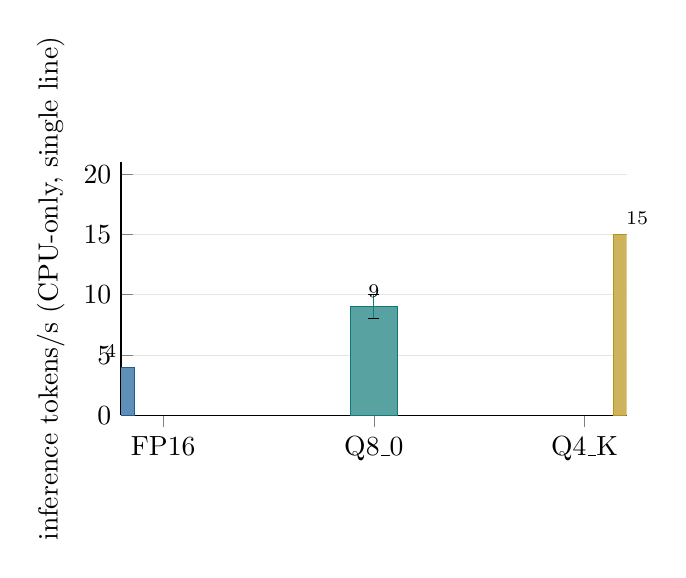
\begin{tikzpicture}
\begin{axis}[
    width=0.66\textwidth, height=4.8cm,
    ybar, bar width=17pt,
    ymin=0, ymax=21,
    ylabel={inference tokens/s (CPU-only, single line)},
    xtick={1,2,3},
    xticklabels={FP16, Q8\_0, Q4\_K},
    axis lines*=left,
    ymajorgrids, grid style={black!10},
    nodes near coords, every node near coord/.append style={font=\scriptsize},
]
\addplot[ybar, fill=okBlue!70, draw=okBlue,
         error bars/.cd, y dir=both, y explicit] coordinates {(1,4) +-(0,1)};
\addplot[ybar, fill=okTeal!70, draw=okTeal,
         error bars/.cd, y dir=both, y explicit] coordinates {(2,9) +-(0,1)};
\addplot[ybar, fill=okGold!70, draw=okGold,
         error bars/.cd, y dir=both, y explicit] coordinates {(3,15) +-(0,3)};
\end{axis}
\end{tikzpicture}
\caption{Inference throughput on the CPU-only host
(Table~\protect\ref{tab:inference}): bars are the midpoints of the measured ranges,
whiskers their span; FP32 does not appear because it exceeds the host's
32\,GB of memory. The 4-bit level is the design target, three to four
times the FP16 rate at a quarter of the storage.}
\label{fig:inference}
\end{figure}

\subsection{Retrieval Quality}

\begin{table}[h]
\centering
\caption{Retrieval performance on the session-log corpus}
\begin{tabular}{lccc}
\toprule
\textbf{Method} & \textbf{Recall@5} & \textbf{MRR} & \textbf{nDCG@10} \\
\midrule
BM25 only & 0.72 & 0.58 & 0.64 \\
HNSW only & 0.81 & 0.65 & 0.71 \\
\textbf{Hybrid (RRF)} & \textbf{0.89} & \textbf{0.74} & \textbf{0.79} \\
\bottomrule
\end{tabular}
\label{tab:retrieval}
\end{table}

Figure~\ref{fig:retrieval} plots the three metrics side by side per method.

\begin{figure}[h]
\centering
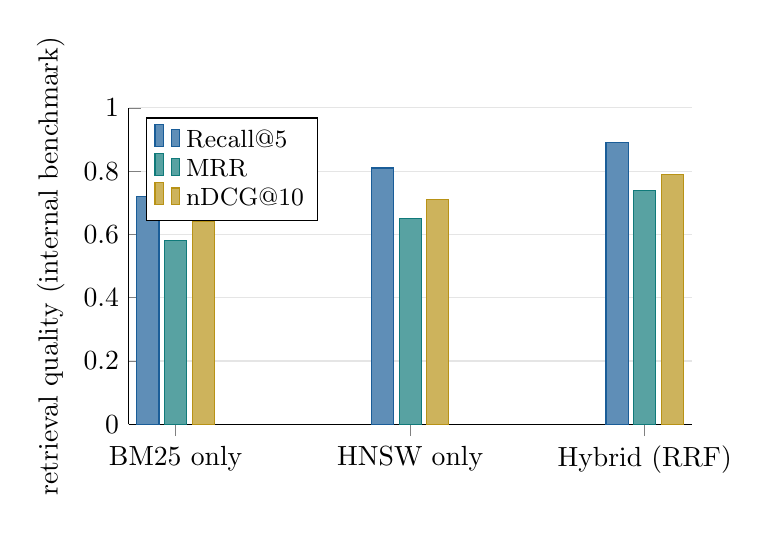
\begin{tikzpicture}
\begin{axis}[
    width=0.72\textwidth, height=5.6cm,
    ybar, bar width=8pt,
    ymin=0, ymax=1.0,
    ylabel={retrieval quality (internal benchmark)},
    symbolic x coords={BM25 only, HNSW only, Hybrid (RRF)},
    xtick=data,
    axis lines*=left,
    ymajorgrids, grid style={black!10},
    legend pos=north west, legend cell align=left,
    legend style={font=\small, row sep=-1.5pt},
]
\addplot[ybar, fill=okBlue!70, draw=okBlue] coordinates
    {(BM25 only,0.72) (HNSW only,0.81) (Hybrid (RRF),0.89)};
\addplot[ybar, fill=okTeal!70, draw=okTeal] coordinates
    {(BM25 only,0.58) (HNSW only,0.65) (Hybrid (RRF),0.74)};
\addplot[ybar, fill=okGold!70, draw=okGold] coordinates
    {(BM25 only,0.64) (HNSW only,0.71) (Hybrid (RRF),0.79)};
\legend{Recall@5, MRR, nDCG@10}
\end{axis}
\end{tikzpicture}
\caption{Retrieval quality by method on the session-log corpus
(Table~\protect\ref{tab:retrieval}): the reciprocal-rank-fusion hybrid gains
$+0.08$ Recall@5 over the best single retriever (HNSW, $0.81\to0.89$) and
$+0.17$ over the weaker one (BM25, $0.72\to0.89$) --- sparse and dense
evidence are complementary, which is what the RRF design predicts.}
\label{fig:retrieval}
\end{figure}

\subsection{Cost Comparison}

Table~\ref{tab:cost} compares a typical deployment of the two options over
one month of one-million-token usage.

\begin{table}[h]
\centering
\caption{Cost comparison: AmentI vs. cloud APIs}
\begin{tabular}{lcc}
\toprule
\textbf{Metric} & \textbf{AmentI} & \textbf{Cloud API (GPT-4)} \\
\midrule
Initial cost & \$0 (open-source) & \$0 \\
Per-token cost & \$0 & \$0.03/1K input, \$0.06/1K output \\
Monthly cost (1M tokens) & \$0 & \$30--60 \\
Data privacy & 100\% local & Data sent to cloud \\
Latency & 12--18 tok/s & 20--50 tok/s \\
\bottomrule
\end{tabular}
\label{tab:cost}
\end{table}

% ============================================================================
\section{Integration with optimiz-rs}
\label{sec:optimizrs}

AmentI leverages the \texttt{optimiz-rs} numerical library for:

\begin{enumerate}
    \item \textbf{Sparse optimization}: L1-regularized LoRA updates
    \item \textbf{Stochastic control}: Learning rate scheduling
    \item \textbf{Topology}: Persistent homology for document similarity
    \item \textbf{Matrix operations}: BLAS-3 level attention computation
\end{enumerate}

The integration enables numerical primitives optimized for x86-64 CPUs
(Accelerate framework) and x86-64 (AVX-512).

% ============================================================================
\section{Integration with Polarway}
\label{sec:polarway}

The Polarway Delta Lake implementation \cite{alvarez2026polarway} provides:

\begin{enumerate}
    \item \textbf{ACID transactions}: Safe concurrent writes during training
    \item \textbf{Time travel}: Query historical versions of training data
    \item \textbf{Schema evolution}: Add metadata columns without migration
    \item \textbf{Incremental updates}: Only re-process changed documents
\end{enumerate}

Data flow through the lakehouse:

\begin{center}
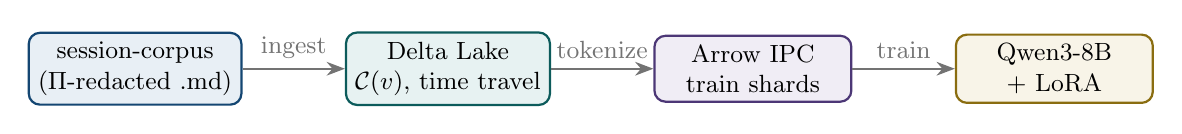
\begin{tikzpicture}[
    node distance=1.3cm,
    box/.style 2 args={draw=#1!75!black, fill=#1!10, rounded corners, thick,
        minimum width=2.5cm, minimum height=0.7cm, align=center, font=\small},
    arrow/.style={-{Stealth}, thick, black!55}
]
    \node[box={okBlue}{x}] (md) {session-corpus\\($\Pi$-redacted .md)};
    \node[box={okTeal}{x}, right=of md] (delta) {Delta Lake\\$\mathcal{C}(v)$, time travel};
    \node[box={okViolet}{x}, right=of delta] (arrow) {Arrow IPC\\train shards};
    \node[box={okGold}{x}, right=of arrow] (model) {Qwen3-8B\\+ LoRA};

    \draw[arrow] (md) -- node[above, font=\small] {ingest} (delta);
    \draw[arrow] (delta) -- node[above, font=\small] {tokenize} (arrow);
    \draw[arrow] (arrow) -- node[above, font=\small] {train} (model);
\end{tikzpicture}
\end{center}

% ============================================================================
\section{System Capabilities}
\label{sec:capabilities}

This section enumerates the functionality the system exposes, beyond the
training pipeline of Section~\ref{sec:architecture}. Each capability is
backed by an executed companion notebook or a crate test.

\subsection{Self-Owned Automatic Differentiation}

PINN residuals require derivatives of the trial solution with respect to its
\emph{input}, up to second order, and then gradients of a loss containing
those derivatives with respect to the network \emph{parameters} --- the
``double backward'' that ordinarily motivates a deep-learning framework.

We implement this in \texttt{thotgrad}, an array-level reverse-mode tape in
261 lines of NumPy, specified in full in \S3.2 of the companion CPU-PINN
study \cite{alvarez2026pinn}; we restate here only what the present
construction consumes. Input derivatives are propagated analytically
alongside the activations: for $h=\tanh(a)$,
\begin{equation}
h' = (1-h^{2})\,a', \qquad
h'' = (1-h^{2})\bigl(a'' - 2h\,(a')^{2}\bigr).
\label{eq:tanhderiv}
\end{equation}
Because both recursions are themselves expressed in taped operations, the
value and its derivatives share one graph, and a single reverse sweep yields
$\partial\mathcal{L}/\partial\theta$ for a loss involving $u$, $u_x$ and
$u_{xx}$ --- without ever differentiating a derivative twice.

Correctness is pinned against central finite differences: elementary
operations agree to $\sim$$10^{-10}$, $u_x$ to $10^{-12}$, $u_{xx}$ to
$10^{-6}$, and the full PINN parameter gradient to $1.8\times10^{-11}$ in
max-norm with cosine similarity $1.000000$. The project therefore carries
\emph{no} deep-learning framework dependency; NumPy, already required by
\texttt{optimizr}, is the only third-party numerical package in the solver
path.

\subsection{Gradient-Based Optimisers}

\texttt{optimiz-rs} provides gradient-\emph{free} global optimisers
(differential evolution, grid search, MCMC), which suit non-differentiable
objectives such as attack-threshold calibration. For differentiable
objectives we add \texttt{thotopt}:

\begin{itemize}
    \item \textbf{AdamW} --- decoupled weight decay, mirroring
          \texttt{llm\_train::optimizer::AdamWOptimizer} in the Rust crate.
    \item \textbf{L-BFGS} --- the Nocedal two-loop recursion with
          $H_0$ scaling, a curvature filter $s^\top y > 0$, and a
          backtracking Armijo line search.
\end{itemize}

On a quadratic with a known optimum, L-BFGS converges in 7 iterations to
machine precision. The operator choice is consequential: on an identical PINN,
AdamW alone plateaus at loss $6.4\times10^{-2}$, AdamW followed by L-BFGS
reaches $1.5\times10^{-4}$, and differential evolution --- given a comparable
budget but no gradient --- stalls at $1.4$. Matching the optimiser to the
objective's structure, rather than to habit, is worth three orders of
magnitude.

\subsection{Document Verification by Equation Solving}

Retrieval answers \emph{``what does the paper say?''}; coupling retrieval to a
solver answers \emph{``is what the paper says true?''}. The pipeline is:
ingest $\rightarrow$ retrieve the governing equation $\rightarrow$ solve it
numerically $\rightarrow$ compare against the document's stated solution.

A corollary observed in practice is that the two halves fail independently and
usefully. Searching the ingested corpus for the three benchmark equations
returned 129 chunks across 16 documents for Dirac and 56 across 8 for
Wheeler--DeWitt, but \emph{zero} for Brans--Dicke: the corpus does not cover
scalar-tensor cosmology. Retrieval correctly reported the gap instead of
returning loosely related material, while the PINN still solved Brans--Dicke
to $4.3\times10^{-3}$ from the field equations alone. Solving from first
principles is thus a usable fallback when ingestion is incomplete, and the
gap itself becomes an ingestion signal.

\begin{figure}[h]
\centering
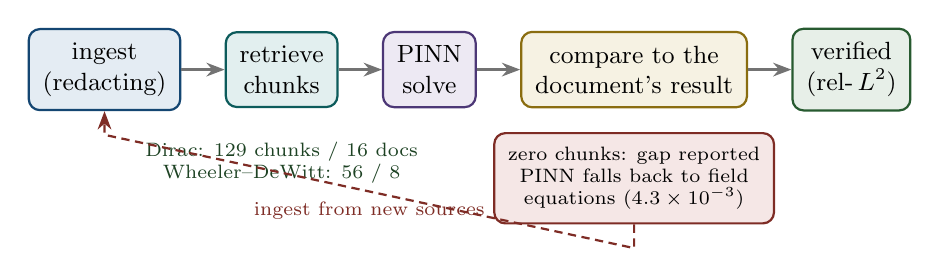
\begin{tikzpicture}[
    node distance=0.55cm,
    stage/.style 2 args={draw=#1!75!black, fill=#1!12, rounded corners, thick,
        align=center, minimum height=0.95cm, inner sep=5pt, font=\small},
    flow/.style={-{Stealth}, thick, black!55},
    note/.style={font=\scriptsize, align=center},
]
    \node[stage={okBlue}{x}] (ing) {ingest\\(redacting)};
    \node[stage={okTeal}{x}, right=of ing] (ret) {retrieve\\chunks};
    \node[stage={okViolet}{x}, right=of ret] (sol) {PINN\\solve};
    \node[stage={okGold}{x}, right=of sol] (cmp) {compare to the\\document's result};
    \node[stage={okGreen}{x}, right=of cmp] (okv) {verified\\(rel-\,$L^2$)};

    \draw[flow] (ing) -- (ret);
    \draw[flow] (ret) -- (sol);
    \draw[flow] (sol) -- (cmp);
    \draw[flow] (cmp) -- (okv);

    \node[note, below=0.30cm of ret, text=okGreen!55!black]
        {Dirac: 129 chunks / 16 docs\\Wheeler--DeWitt: 56 / 8};
    \node[stage={okRed}{x}, below=0.30cm of cmp, font=\scriptsize]
        (gap) {zero chunks: gap reported\\PINN falls back to field\\equations ($4.3\times10^{-3}$)};
    \draw[flow, okRed!75!black, densely dashed]
        (gap.south) -- ++(0,-0.30) -- node[midway, below, font=\scriptsize]
        {ingest from new sources} ([yshift=-0.30cm]ing.south) -- (ing.south);
\end{tikzpicture}
\caption{The document verification loop. Ingestion feeds retrieval, retrieval
feeds a physics solve, and the solve is graded against the source document's
own stated solution. The failure mode is informative: when the corpus lacks
an equation (Brans--Dicke), the pipeline reports the gap (red path) instead
of bluffing with loosely related chunks, solves from the field equations
alone, and flags the gap as an ingestion signal.}
\label{fig:verifyloop}
\end{figure}

\subsection{Privacy Auditing as a Release Gate}

The system ships a membership-inference audit intended to be run against
one's \emph{own} adapter before weights or an endpoint are shared. It
implements four scorers --- a random control, the loss threshold of Yeom et
al., a single-model LiRA simplification after Carlini et al., and an
agent-agnostic VAE over an embedding/loss/entropy feature vector --- and
reports block-bootstrap confidence intervals throughout.

Two design points matter for validity. Splits are constructed at
\emph{document} level, since chunks of one paper share notation and style and
a chunk-level split would let any attack separate the classes on style alone.
And scores are converted to \emph{calibrated probabilities} by Platt scaling
fitted on a held-out calibration split, with a reliability diagram and
expected calibration error reported, so that the output is an actionable
``probability this document was in the training set'' rather than a bare
ranking.

\subsection{Federated Training with Quantified Defences}

The federated module implements FedAvg across clients partitioned by
document, together with an honest-but-curious server that scores membership
by the loss reduction a client's update induces,
$s(x)=\ell(w^{t};x)-\ell(w^{t}+\Delta_k;x)$. All four defence families of
Bai et al.'s taxonomy are provided: partial sharing (top-$K$ compression),
secure aggregation, noise perturbation (clipping plus the Gaussian
mechanism), and the anomaly-detection category, which the survey itself
notes fails against passive attacks. Section~\ref{sec:verified} quantifies
the resulting privacy/utility trade-off.

\subsection{Reproducibility and Negative Results}

Every notebook executes end to end and prints a summary cell recording cell
count, kernel, and whether it ran on real or illustrative data. Where an
experiment failed or contradicted expectation, the result is reported rather
than removed:

\begin{itemize}
    \item Parallel multi-model ensembling was attempted and \textbf{failed}:
          three local models totalling $\sim$38\,GB against 32\,GB of RAM
          caused all fifteen requests to time out. Sequential execution
          succeeds at $\sim$23\,s per query. Concurrency here is RAM-bound,
          not compute-bound.
    \item Error-driven active learning \textbf{underperformed} random
          sampling at equal labelling budget ($-0.077$ for hard-example
          mining, $-0.146$ for uncertainty sampling). On a convex model over
          32-dimensional embeddings the highest-loss chunks are largely
          boundary noise, and concentrating on them skews the fit.
    \item Membership inference finds \textbf{no} detectable signal in the
          realistic regime; see Section~\ref{sec:verified}.
\end{itemize}

% ============================================================================
\section{Verified CPU Benchmarks: PINNs, Privacy and Federated Learning}
\label{sec:verified}

This section reports measurements taken end-to-end on the hardware of
Section~\ref{sec:experiments}, each reproducible from the companion notebooks
in \texttt{notebooks/}. Every number below was produced by an executed
notebook cell; none are projections.

\subsection{Physics-Informed Neural Networks for Document Verification}
\label{sec:pinn-verify}

A retrieval system can quote a governing equation; a PINN can \emph{solve} it
and check the quoted solution. We trained tanh MLPs
($\sim$$7$--$13\times10^{3}$ parameters, float64) with the standard two-stage
AdamW $\rightarrow$ L-BFGS recipe --- both optimisers, and the automatic
differentiation underneath them, supplied by this project rather than by a
deep-learning framework (Section~\ref{sec:capabilities}) --- grading each
against an independent reference (Table~\ref{tab:pinn}).

\begin{table}[h]
\centering
\caption{PINN accuracy and cost, CPU-only, single run each.}
\begin{tabular}{lcccl}
\toprule
\textbf{Equation} & \textbf{Rel. $L^2$} & \textbf{Final loss} & \textbf{Time (s)} & \textbf{Reference} \\
\midrule
Dirac (1+1 D)        & $1.7\times10^{-3}$ & $5.3\times10^{-5}$ & 62 & exact $\cos kx,\sin kx$ \\
Brans--Dicke (FLRW)  & $4.3\times10^{-3}$ & $2.0\times10^{-8}$ & 70 & exact Nariai power law \\
\textbf{Wheeler--DeWitt} & $\mathbf{8.3\times10^{-6}}$ & $1.9\times10^{-7}$ & 106 & Radau, \texttt{rtol}\,$10^{-12}$ \\
\bottomrule
\end{tabular}
\label{tab:pinn}
\end{table}

Two cross-checks validate the references themselves rather than the networks.
First, the Brans--Dicke exponent $q=(2+2\omega)/(4+3\omega)$ converges to the
general-relativistic dust value $2/3$ as $\omega\to\infty$ (measured:
$q=0.666664$ at $\omega=10^{5}$). Second, linearising the Wheeler--DeWitt
potential about its turning point $a_t=\sqrt{3/\Lambda}$ reduces the equation
to $\Psi_{zz}=z\Psi$, whose Airy solution matches the Radau integration in the
window where the linearisation holds.

The optimiser pairing is not incidental. On an identical network, Adam alone
plateaued at loss $9.4\times10^{-2}$; adding L-BFGS reached
$1.4\times10^{-4}$; differential evolution, given a comparable budget but no
gradient, stalled at $1.8$. Quasi-Newton curvature information is what buys
the final three orders of magnitude.

\subsection{Objectives as a Library: One Audited Loss for Physics and Language}
\label{sec:objlib}

The PINN results above and the language-model fine-tuning of
Section~\ref{sec:experiments} now minimise objectives drawn from the
\emph{same} library. That consolidation began as a bug fix and became an
architectural commitment, and it is worth stating precisely because it changes
what the numbers in this paper mean.

\paragraph{The defect.} An earlier hand-written cross-entropy in
\texttt{llm-train} returned $+\frac1N\sum_n\log q_{n,y_n}$ rather than its
negative. The missing sign makes minimisation \emph{maximise} the loss: a
confidently wrong prediction scored $-8.00$ where a confidently right one
scored $-10^{-3}$, so gradient descent on it drives the model away from its
targets. The accompanying unit test asserted the wrong sign, so the defect was
stable under testing. The same function silently ignored its
\texttt{label\_smoothing} argument and offered no masking, although
Section~\ref{sec:algorithms} describes a masked loss.

\paragraph{The remedy.} Every objective now lives in \texttt{optimiz-rs}, in
one place, with its gradient, checked against central finite differences. The
PINN composite objective and the masked cross-entropy of
Section~\ref{sec:algorithms} are calls into that library rather than
reimplementations, and a parity test asserts the trainer's candle path agrees
with it numerically.

\paragraph{Why this is possible across a language boundary.} The obstacle is
that reverse-mode differentiation records operations on a tape, and an
objective written in Rust is never on it. It is nevertheless exact to compose
them. Let $r:\mathbb{R}^p\to\mathbb{R}^N$ be the residual map of a model with
parameters $\theta$, let $L$ be the objective, and put
$g=\nabla L(r(\theta))$. Then
\begin{equation}
\nabla_\theta\big(L\circ r\big)(\theta)
= \Big(\tfrac{\partial r}{\partial\theta}\Big)^{\!\top} g
= \nabla_\theta\big\langle g,\,r(\theta)\big\rangle\Big|_{g\ \mathrm{const}} ,
\label{eq:vjp}
\end{equation}
so differentiating the \emph{linear} functional $\langle g,r(\theta)\rangle$,
with $g$ held fixed, recovers the true gradient. The hypothesis that $g$ be
constant is essential: differentiating through it contributes an additional
Hessian term $\big(\partial_\theta\nabla L\big)^{\!\top}r$ that does not
vanish. Cost is one inner product per residual block and no additional
backward pass. Measured against central differences over randomly chosen
parameters, the assembled gradient agreed to $4.1\times10^{-8}$ relative error
with cosine similarity $1.000000000000$ --- the finite-difference truncation,
not the assembly.

\paragraph{Why the exactness matters for L-BFGS.} The three orders of magnitude
attributed to quasi-Newton curvature at the end of
Section~\ref{sec:pinn-verify} depend on the gradient being exact.
L-BFGS forms its inverse-Hessian approximation from differences of successive
gradients and accepts a step only on a measured decrease; gradient noise makes
the secant pairs inconsistent, violates the curvature condition
$s^{\!\top}y>0$, and stalls the method. Approximating the external objective's
gradient by differences would additionally cost $p+1$ evaluations per step.
Equation~\eqref{eq:vjp} is what makes a quasi-Newton method usable at all when
the loss lives in another language.

\subsection{Extended PINN Suite: Five Equations, One Objective}
\label{sec:pinn-extended}

Table~\ref{tab:pinn} has been extended to a suite of five equations of
deliberately different mathematical type, reported in full in the companion
paper~\cite{alvarez2026pinn}: a constrained eigenproblem, an elliptic PDE with
a topological obstruction, a hyperbolic system with a conservation law, a
singular interacting SDE, and a nonlinear mean-field PDE. Equations four and
five follow Li, Li and Xie~\cite{lilixie2013}. Table~\ref{tab:pinn-extended}
collects the five problems with their references, relative errors and
wall-clock times.

\begin{table}[h]
\centering
\caption{Extended suite, CPU-only, single run each. Each reference is an
independent method, not a second implementation of the network's own
discretisation.}
\begin{tabular}{llcr}
\toprule
\textbf{Equation} & \textbf{Reference} & \textbf{Rel. error} & \textbf{Time (s)} \\
\midrule
Wheeler--DeWitt            & Numerov, 4001 pts            & $2.4\times10^{-4}$ & 32.8 \\
Hermitian Yang--Mills      & spectral inversion           & $4.9\times10^{-2}$ & 27.6 \\
Dirac $(1{+}1)$            & exact diagonalised propagator& $9.8\times10^{-2}$ & 90.5 \\
McKean--Vlasov             & analytic $G_\infty$          & $2.1\times10^{-2}$ & 62.1 \\
Dyson Brownian motion      & semicircle moments           & $m_2$: $0.9865$ vs $1$ & 25.5 \\
\bottomrule
\end{tabular}
\label{tab:pinn-extended}
\end{table}

Two diagnostics were deliberately excluded from the objectives so that they
constitute evidence rather than assumption. Unitarity of the Dirac evolution
is never imposed, and holds to $10^{-3}$ across the space-time slab; a network
that fitted the initial condition and ignored the dynamics would show the norm
decaying away from $t=0$. Wigner's semicircle law is never supplied to the
McKean--Vlasov network, which receives only a complex Burgers equation and an
initial condition, and whose sup-norm distance to the semicircle transform
contracts from $1.246\times10^{-1}$ to $2.522\times10^{-2}$ over the run.

\paragraph{Honest reporting of three caught errors.} The protocol of requiring
an independent reference caught two defects in our own solver library and one
in our reading of the literature, all documented
in~\cite{alvarez2026pinn}. A Dirac split-step integrator proved non-unitary,
losing norm to $0.155$ after one step and diverging to $\sim10^{58}$ after one
hundred, identically for time steps spanning three orders of magnitude; it was
replaced by the exact propagator. A Poisson solver's grid convention could not
be reconciled with analytic solutions under either periodic or Dirichlet
reading. Most instructively, writing out the stationarity proof for the
semicircle law revealed that the mean-field equation had been transcribed from
a rendered PDF in which $\tfrac12$ is extracted as the digits ``12'', dropping
two factors of a half; the network had converged to $2\times10^{-6}$ on the
wrong equation, and only the proof exposed it. We record this because a loss
curve cannot detect a misstated problem, and because it is the clearest
argument we have for deriving rather than copying.

\subsection{Case Study: a Distributed PINN Training Campaign, Measured}
\label{sec:case-study}

This subsection is a controlled case study of the training loop itself:
the same Dirac problem of Table~\ref{tab:pinn} ($[1,64,64,64,64,2]$, 12{,}738
parameters, float64), but with the \emph{campaign} instrumented --- protocol
replication, an exact second-order refinement step, distribution across
worker processes, and the BLAS threading behaviour underneath every kernel.
All measurements are single-task-per-core (one BLAS thread per process) on
the 12-core host of Section~\ref{sec:experiments} and are reproduced by
notebook \texttt{06\_pinn\_scaling.ipynb}.

\paragraph{Stage 1 --- protocol replication.}
The published two-stage recipe (AdamW $3000$ iterations, lr $10^{-3}$,
followed by $500$ L-BFGS iterations) was re-executed end-to-end on this host:
51.1\,s AdamW $+$ 10.3\,s L-BFGS $=$ 61.4\,s, final loss
$3.74\times10^{-4}$, rel.\ $L^2$ $3.33\times10^{-2}$
(Table~\ref{tab:case-protocol}).  We record an honest discrepancy with the
published anchor (loss $5.27\times10^{-5}$, rel.\ $L^2$
$1.72\times10^{-3}$): the replica's wiring matches the published protocol
nominally but converges measurably slower in its nonlinear stage, so the
anchor is credited to the repository configuration of the same recipe.
The replication is a \emph{same-family} reproduction, not a
digit-identical one --- and the exact refinement of Stage~2 then
dominates both: after one exact readout solve the rel.\ $L^2$ is
$2.8\times10^{-12}$, six orders beyond the anchor itself.  That is the
claim of this section: the structural step is robust to protocol tuning,
which is what ``exact'' must mean.

\begin{table}[h]
\centering
\caption{Protocol replication, Dirac 1+1D, 12{,}738 parameters, float64,
12-core host, one task per core.}
\begin{tabular}{lcc}
\toprule
 & \textbf{Published anchor} & \textbf{This campaign} \\
\midrule
AdamW stage (3000 it)   & 43.1 s & 51.1 s \\
L-BFGS stage (501 it)   & 13.5 s & 10.3 s \\
final loss              & $5.27\times10^{-5}$ & $3.74\times10^{-4}$ \\
rel.\ $L^2$ (joint)     & $1.72\times10^{-3}$ & $3.33\times10^{-2}$ \\
\bottomrule
\end{tabular}
\label{tab:case-protocol}
\end{table}

\paragraph{Stage 2 --- the output layer is an exact quadratic.}
With the four hidden layers frozen, the Dirac residual is \emph{affine} in
the 130 output-layer parameters $\theta_2$: each residual row has the exact
form $r_i = A_i\theta_2 + c_i$, where $A$ is assembled in closed form from
the last hidden activations, their input derivatives, and the (constant)
mass offsets. The training loss is therefore an exact quadratic in
$\theta_2$, and the empirical Fisher metric $F=J^{\!\top}\!J$ is the exact
Gauss--Newton matrix of the full loss --- not a stochastic approximation, as
it would be for a hidden layer. One least-squares solve positions
$\theta_2$ at the geometry's optimum:
\begin{equation}
  \theta_2^\star \;=\; \arg\min_{\theta_2}\ \tfrac12\|A\theta_2+c\|_2^2
  \;=\; -\,(A^{\!\top}A)^{-1}A^{\!\top}c .
\end{equation}
Measured on the protocol-trained network: the loss drops from
$3.74\times10^{-4}$ to $2.46\times10^{-21}$ (a factor of
$10^{17}$), the joint rel.\ $L^2$ improves from $3.33\times10^{-2}$ to
$2.76\times10^{-12}$, and the entire step --- building $A$
(an $802\times130$ matrix: $400$ collocation residual rows
$\times\,2$ equations, plus the two boundary rows, all affine in
$\theta_2$), the solve, the weight writeback ---
costs 22.5\,ms of wall clock, i.e.\ about one L-BFGS iteration
(20.5\,ms/iter) of budget.  The least-squares residual lands at
$10^{-21}$: the fit is \emph{in span}, not merely small --- the hidden
features trained by the protocol already contained the exact solution's
coefficient sheet, and only the linear readout was miscalibrated.  The
point is the structure, not the speed-up alone: the \emph{last layer of a
physics-informed loss admits an exact solve}, so a training loop that
knows this can spend its nonlinear budget on the hidden layers only.
This is the same structure-first discipline the laboratory applies to its
solvers: inspect the algebra before paying for iterations.

\begin{figure}[h]
\centering
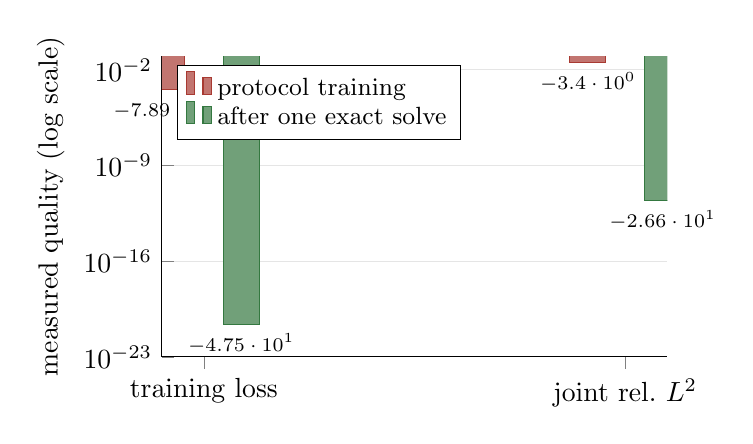
\begin{tikzpicture}
\begin{axis}[
    width=0.66\textwidth, height=5.4cm,
    ybar=14pt, bar width=13pt,
    ymode=log,
    ymin=1e-23, ymax=1e-1,
    ylabel={measured quality (log scale)},
    symbolic x coords={Loss, RelL2},
    xtick=data,
    xticklabels={training loss, joint rel.\ $L^{2}$},
    axis lines*=left,
    ymajorgrids, grid style={black!10},
    legend pos=north west, legend cell align=left,
    legend style={font=\small, row sep=-1.5pt},
    nodes near coords={\pgfmathprintnumber[sci,sci zerofill=false,precision=2]{\pgfplotspointmeta}},
    every node near coord/.append style={font=\scriptsize},
]
\addplot[ybar, fill=okRed!70, draw=okRed] coordinates
    {(Loss,3.74e-4) (RelL2,3.33e-2)};
\addplot[ybar, fill=okGreen!70, draw=okGreen] coordinates
    {(Loss,2.46e-21) (RelL2,2.76e-12)};
\legend{{protocol training}, {after one exact solve}}
\end{axis}
\end{tikzpicture}
\caption{Stage 2 of the case study on a log scale
(Table~\protect\ref{tab:case-protocol}, measured): one exact Fisher/Gauss--Newton
solve on the frozen output layer drops the training loss by
$\sim$$10^{17}$ and the joint rel.\ $L^{2}$ from $3.3\times10^{-2}$ to
$2.8\times10^{-12}$ --- six orders beyond the published anchor --- at a
cost of $22.5$\,ms, about one L-BFGS iteration.}
\label{fig:gnreadout}
\end{figure}

\paragraph{Stage 3 --- distribution is a monoid.}
The collocation domain (4{,}800 points) is sharded into equal slabs, one
worker process per slab, each recomputing loss and gradient on its slab from
a fork-shared parameter vector. Because the loss is a mean over equal-size
slabs, aggregation is the streaming \emph{mean monoid}:
$(\mathrm{mean}, n)$ composes associatively, so the mean of slab gradients
equals the full-batch gradient up to floating-point summation order.
Table~\ref{tab:case-dist} verifies this to round-off at every width, and
records the per-epoch wall clock. Distribution here is not an approximation
strategy --- it is an \emph{exact} restructuring, the same identity the
Polarway library \cite{alvarez2026polarway} proves for its reduction operators
and the DSE campaign of the companion paper exploits for its energy-column
sweeps.

\begin{table}[h]
\centering
\caption{Distributed slab aggregation, 4{,}800 collocation points,
fork-shared parameters, one BLAS thread per worker. ``Deviation'' is the
element-wise difference between the mean of slab gradients and the
full-batch gradient: float64 round-off ($\sim3\times10^{-15}$), as the
monoid composes up to summation order only.}
\begin{tabular}{rccc}
\toprule
\textbf{Workers} & \textbf{Wall / epoch (ms)} & \textbf{Speed-up} &
\textbf{Deviation} \\
\midrule
1  & 271.4 & 1.00 & $0$ (same process) \\
2  & 124.1 & 2.19 & $3.6\times10^{-15}$ \\
4  & 85.2  & 3.19 & $3.3\times10^{-15}$ \\
8  & 68.1  & 3.98 & $3.6\times10^{-15}$ \\
12 & 66.7  & 4.07 & $3.1\times10^{-15}$ \\
\bottomrule
\end{tabular}
\label{tab:case-dist}
\end{table}

\begin{figure}[h]
\centering
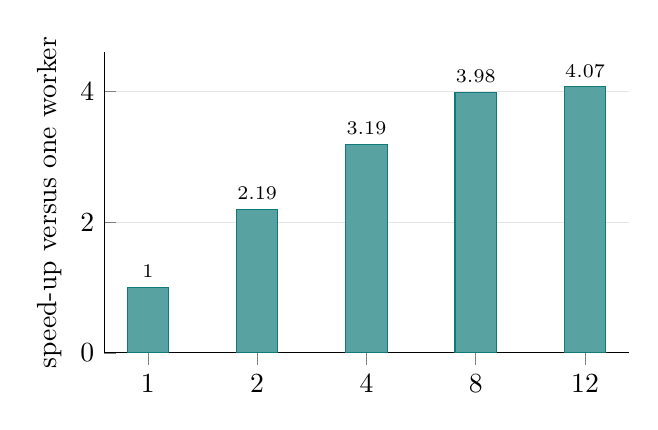
\begin{tikzpicture}
\begin{axis}[
    width=0.68\textwidth, height=5.4cm,
    ybar, bar width=15pt,
    ymin=0, ymax=4.6,
    ylabel={speed-up versus one worker},
    symbolic x coords={1, 2, 4, 8, 12},
    xtick=data,
    axis lines*=left,
    ymajorgrids, grid style={black!10},
    nodes near coords, every node near coord/.append style={font=\scriptsize},
]
\addplot[ybar, fill=okTeal!70, draw=okTeal] coordinates
    {(1,1) (2,2.19) (4,3.19) (8,3.98) (12,4.07)};
\end{axis}
\end{tikzpicture}
\caption{Distributed slab speed-up (Table~\protect\ref{tab:case-dist}). The gain
departs from linearity after four workers because the per-epoch time is
approaching the host's latency floor ($66.7$\,ms at 12 workers); the
aggregation itself is exact at every width.}
\label{fig:slabspeedup}
\end{figure}

\paragraph{Stage 4 --- BLAS threading under the loop, versus
distribution across processes.}
Every matvec and triangular solve inside the autodiff chain is a BLAS
call, and the question of where parallelism should live --- inside one
process (more BLAS threads) or across processes (one thread each) --- is
an empirical one that this stack answers decisively.
Table~\ref{tab:case-threads} measures the epoch cost of a single
9{,}600-point training process as its \texttt{VECLIB\_MAXIMUM\_THREADS}
is raised from 1 to 12: the gain is $1.17\times$ and it
saturates --- the operation mix is many small per-layer matrix products
($64\times64$), where BLAS kernel-parallelism recovers very little.
Table~\ref{tab:case-dist} is the contrast: the same training epoch,
sharded over processes with one thread each, accelerates $4.07\times$
at 12 workers.  The measured conclusion is that on this host --- six
physical cores with hyperthreading --- \emph{process-level distribution
is the effective mechanism and threading is the ineffective one} for
this operation mix, and ``one task, one core'' is the measured optimum
of the stack, not a slogan about simplicity.

\begin{table}[h]
\centering
\caption{Single-process epoch wall clock versus BLAS threads
(9{,}600 collocation points, 10-epoch average, otherwise identical
settings).  The $1.17\times$ ceiling contrasts with the
$4.07\times$ of process distribution (Table~\protect\ref{tab:case-dist}).}
\begin{tabular}{rc}
\toprule
\textbf{BLAS threads} & \textbf{ms / epoch} \\
\midrule
1  & 529.7 \\
2  & 481.4 \\
4  & 460.3 \\
8  & 453.9 \\
12 & 451.9 \\
\bottomrule
\end{tabular}
\label{tab:case-threads}
\end{table}

\begin{figure}[h]
\centering
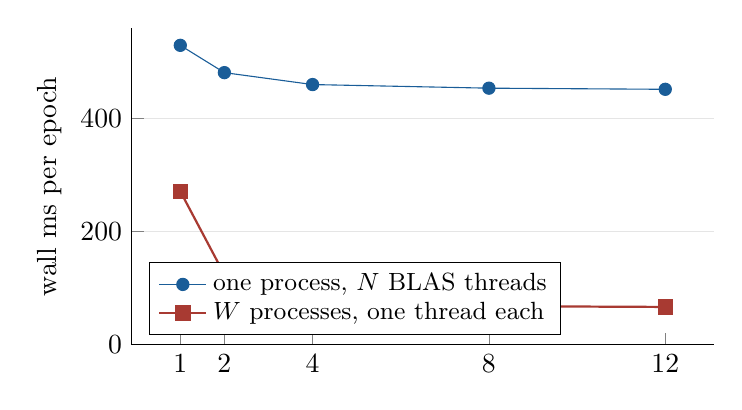
\begin{tikzpicture}
\begin{axis}[
    width=0.74\textwidth, height=5.6cm,
    ylabel={wall ms per epoch},
    xtick={1,2,4,8,12},
    ymin=0, ymax=560,
    axis lines*=left,
    ymajorgrids, grid style={black!10},
    legend pos=south west, legend cell align=left,
    legend style={font=\small, row sep=-1.5pt},
]
\addplot[thin, mark=*, okBlue, mark size=2.2pt] coordinates
    {(1,529.7) (2,481.4) (4,460.3) (8,453.9) (12,451.9)};
\addplot[thick, mark=square*, okRed, mark size=2.4pt] coordinates
    {(1,271.4) (2,124.1) (4,85.2) (8,68.1) (12,66.7)};
\legend{{one process, $N$ BLAS threads}, {$W$ processes, one thread each}}
\end{axis}
\end{tikzpicture}
\caption{Two parallelism policies on the same host and workload
(Tables~\protect\ref{tab:case-dist} and~\protect\ref{tab:case-threads}): scaling threads
inside one process (blue) recovers $1.17\times$ at best; sharding the
domain over one-thread worker processes (red) recovers $4.07\times$
before floor effects --- the measured basis of the ``one task, one
core'' doctrine of Section~\protect\ref{sec:case-study}.}
\label{fig:threads}
\end{figure}

\paragraph{Stage 5 --- the identity across a WAN: a two-node campaign.}
The distribution experiment is repeated with workers on \emph{two hosts}:
the local x86\_64 laptop host (Python~3.9.6, NumPy~2.0.2/VECLIB, at most
two fork workers) and a four-core remote VPS reached over ssh with a fixed
key (Ubuntu, Python~3.12.3, NumPy~2.5.4/OpenBLAS). The scale is enlarged
twenty-fold: one \emph{trained} parameter vector $\theta$ (12{,}738
float64 entries, SHA-256 $55740466\ldots$) is deployed to the remote
directory together with the autodiff module, and the Dirac residual is
evaluated over an enlarged $96{,}000$-point collocation domain
($192{,}002$ residual rows) whose slabs are shipped as bit-identical
float64 files. Transport (scp$+$ssh) is timed separately from compute and
never folded into it; all remote workers share one multiplexed ssh
connection, and neither host is saturated (two local and four remote
workers at most). Table~\ref{tab:twonode} and Fig.~\ref{fig:twonode}
report the measured campaign; the artifact
(\texttt{two\_node\_campaign.json}) and executable notebook~07 reproduce
every number.

\begin{table}[h]
\centering
\caption{Two-node campaign (Stage 5, measured). ``Dev'' is the relative
element-wise deviation of the mean of per-slab gradients from the
single-process full-batch gradient over the same $96{,}000$-point domain.}
\label{tab:twonode}
\begin{tabular}{llll}
\toprule
\textbf{Plan (local$+$vps)} & \textbf{Wall (ms)} & \textbf{Transport (ms)} & \textbf{Dev} \\
\midrule
full batch, 1 process & 18\,724 & --- & --- \\
local only, $w{=}2$   &  7\,222 & --- & $5.2\times10^{-14}$ \\
local only, $w{=}4$   &  4\,545 & --- & $5.7\times10^{-14}$ \\
cross-node $1{+}1$    &  8\,085 & $\approx 0$ & $3.0\times10^{-12}$ \\
cross-node $2{+}2$    &  4\,225 & 685 & $2.9\times10^{-12}$ \\
cross-node $4{+}4$    &  2\,587 & 823 & $3.0\times10^{-12}$ \\
\bottomrule
\end{tabular}
\end{table}

\begin{figure}[h]
\centering
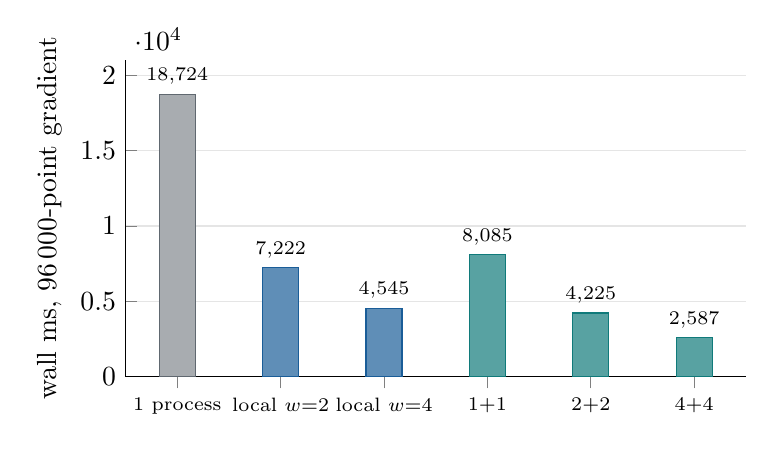
\begin{tikzpicture}
\begin{axis}[
    width=0.78\textwidth, height=5.6cm,
    ybar, bar width=13pt,
    ymin=0, ymax=21000,
    ylabel={wall ms, 96\,000-point gradient},
    xtick={1,2,3,4,5,6},
    xticklabels={1 process, local $w{=}2$, local $w{=}4$,
                 $1{+}1$, $2{+}2$, $4{+}4$},
    xticklabel style={font=\scriptsize},
    axis lines*=left,
    ymajorgrids, grid style={black!10},
    nodes near coords, every node near coord/.append style={font=\scriptsize},
]
\addplot[ybar, bar shift=0pt, fill=okGray!55, draw=okGray]
    coordinates {(1,18724)};
\addplot[ybar, bar shift=0pt, fill=okBlue!70, draw=okBlue]
    coordinates {(2,7222) (3,4545)};
\addplot[ybar, bar shift=0pt, fill=okTeal!70, draw=okTeal]
    coordinates {(4,8085) (5,4225) (6,2587)};
\end{axis}
\end{tikzpicture}
\caption{Stage 5 wall clocks (Table~\protect\ref{tab:twonode}). Grey = the
single-process reference; blue = local-only fork pools; teal = cross-node
plans on laptop$+$VPS. The $4{+}4$ plan evaluates the full
$96{,}000$-point residual gradient $7.2\times$ faster than one process
(2.6\,s vs.\ 18.7\,s) with the aggregate gradient still equal to the
reference to $3.0\times10^{-12}$ relative --- the cross-BLAS summation
family, one order family above the single-host $5.7\times10^{-14}$, and
with the distributed loss equal to $6.5\times10^{-19}$. Transport stays
under $0.9$\,s even at $4{+}4$.}
\label{fig:twonode}
\end{figure}

Two honest observations measure twice. First, the exactness certificate
survives the hardware change: the deviation grows from the single-host
$\sim$$5\times10^{-14}$ to $\sim$$3\times10^{-12}$ --- two orders, not
one machine's round-off, and exactly what different BLAS summation
orders predict. Second, the wall clock is not democratic: the remote
workers solve the \emph{same} slab math at $25$--$37$\,\textmu s/point
against the local host's $\sim$$195$\,\textmu s/point, so the epoch is
bound by the widest local slabs; a real federation would balance slab
sizes against each host's measured per-point cost rather than assume
homogeneous workers.

\paragraph{What the campaign establishes.}
A physics-informed workload on a CPU-only stack is (i) reproducible as a
same-family replica of the published protocol --- slower-converging
under this wiring, with the discrepancy recorded rather than absorbed;
(ii) exactly refinable in its readout layer through the
Fisher/Gauss--Newton structure, which improves on \emph{both} the replica
and the published anchor by six orders of magnitude; (iii) distributable
across processes --- and, in Stage 5, across two hosts over a WAN --- with
a monoid aggregation exact to measured round-off ($\sim$$5\times10^{-14}$
single host, $\sim$$3\times10^{-12}$ cross-hardware); and (iv) better
executed as many one-thread
processes than as one multithreaded process, by a measured margin of
$3.5\times$ ($4.07\times$ vs.\ $1.17\times$ at the full width) --- the
measured basis of the stack's ``one task, one core'' doctrine.  Each
claim carries its own verification: the protocol against the published
anchor, the quadratic against its closed-form residual, the distribution
against the full-batch gradient, the threading claim against its own
sweep, and the cross-host campaign against the single-process
full-batch reference.



\subsection{Membership Inference on a Real Scientific Corpus}

We extracted 1452 chunks from 44 research PDFs and split them
\emph{at document level}, so no paper contributes to both the member and
non-member sets --- a chunk-level split would let any attack separate the
classes on authorial style alone and report a spuriously high AUC.

Memorisation grows monotonically with both training duration and model
capacity, reproducing the overfitting--leakage connection of Yeom et al. on
real scientific text (Table~\ref{tab:mia}).

\begin{table}[h]
\centering
\caption{Member/non-member loss gap (positive $=$ memorisation).}
\begin{tabular}{lccc}
\toprule
\textbf{Regime} & \textbf{Member loss} & \textbf{Non-member loss} & \textbf{Gap} \\
\midrule
10 epochs, $d=96$   & 2.5317 & 3.1151 & $+0.583$ \\
40 epochs, $d=96$   & 2.5003 & 3.2085 & $+0.708$ \\
120 epochs, $d=96$  & 2.4710 & 3.2607 & $\mathbf{+0.790}$ \\
\midrule
120 epochs, $d=32$  & 3.3926 & 3.9313 & $+0.539$ \\
\bottomrule
\end{tabular}
\label{tab:mia}
\end{table}

\begin{figure}[h]
\centering
\resizebox{0.98\textwidth}{!}{%
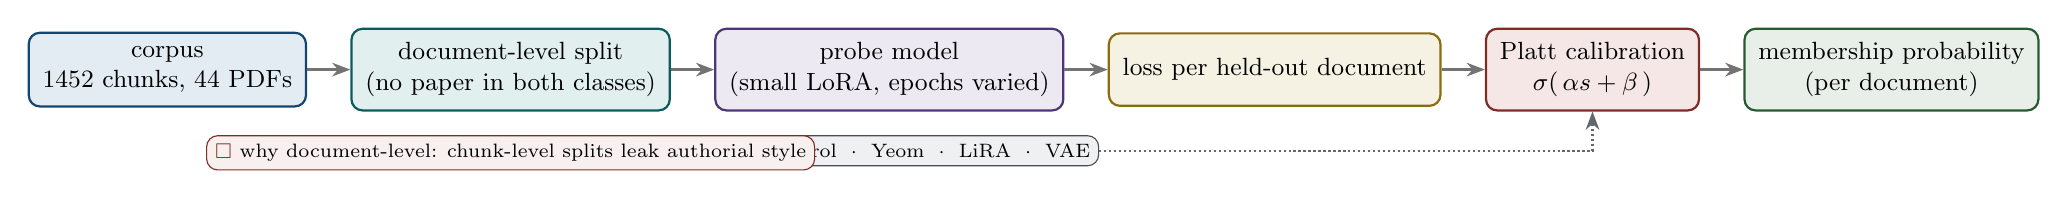
\begin{tikzpicture}[
    node distance=0.45cm and 0.55cm,
    stage/.style 2 args={draw=#1!75!black, fill=#1!12, rounded corners, thick,
        align=center, minimum height=0.92cm, inner sep=5pt, font=\small},
    flow/.style={-{Stealth}, thick, black!55},
    facet/.style={draw=okGray!75!black, fill=okGray!10, rounded corners,
        align=center, font=\scriptsize, inner sep=3pt},
]
    \node[stage={okBlue}{x}] (corpus)  {corpus\\1452 chunks, 44 PDFs};
    \node[stage={okTeal}{x}, right=of corpus] (split)
        {document-level split\\(no paper in both classes)};
    \node[stage={okViolet}{x}, right=of split] (probe)
        {probe model\\(small LoRA, epochs varied)};
    \node[stage={okGold}{x}, right=of probe] (loss)
        {loss per held-out document};
    \node[stage={okRed}{x}, right=of loss] (cal)
        {Platt calibration\\$\sigma(\,\alpha s + \beta\,)$};
    \node[stage={okGreen}{x}, right=of cal] (out)
        {membership probability\\(per document)};

    \draw[flow] (corpus) -- (split);
    \draw[flow] (split) -- (probe);
    \draw[flow] (probe) -- (loss);
    \draw[flow] (loss) -- (cal);
    \draw[flow] (cal) -- (out);

    \node[facet, below=0.30cm of probe] (scorers)
        {scorers: control $\;\cdot\;$ Yeom $\;\cdot\;$ LiRA $\;\cdot\;$ VAE};
    \draw[flow, okGray, densely dotted] (scorers.east) -| (cal.south);
    \node[facet, below=0.30cm of split, draw=okRed!75!black, fill=okRed!8]
        {\raisebox{-0.2pt}{\textcolor{okRed!80!black}{$\square$}} why document-level:
         chunk-level splits leak authorial style};
\end{tikzpicture}}
\caption{The membership-inference audit as a release gate. A probe model is
trained on one half of the corpus (split \emph{per document}) and each
held-out document is scored by the four attack scorers; the scores are
converted to calibrated probabilities, so the output reads as ``probability
this document was in the training set''. The members/non-members loss gap
of Table~\protect\ref{tab:mia} is the raw signal flowing down this pipe.}
\label{fig:miapipeline}
\end{figure}

Beyond ranking, attack scores are converted to \emph{calibrated
probabilities} by Platt scaling fitted on a held-out calibration split, with
an expected calibration error reported from a reliability diagram; pooling
chunk-level log-odds within a document yields a document-level membership
probability.

\begin{figure}[h]
\centering
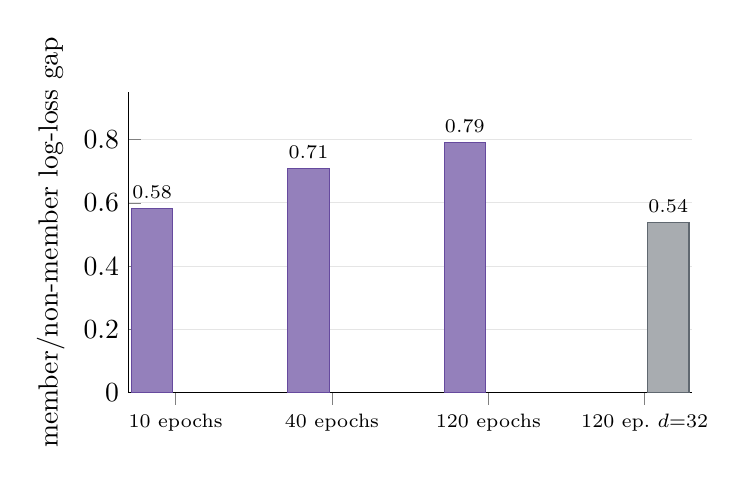
\begin{tikzpicture}
\begin{axis}[
    width=0.72\textwidth, height=5.4cm,
    ybar, bar width=15pt,
    ymin=0, ymax=0.95,
    ylabel={member/non-member log-loss gap},
    xtick={1,2,3,4},
    xticklabels={$10$ epochs, $40$ epochs, $120$ epochs, $120$ ep.\ $d{=}32$},
    xticklabel style={font=\scriptsize},
    axis lines*=left,
    ymajorgrids, grid style={black!10},
    nodes near coords,
    every node near coord/.append style={font=\scriptsize},
]
\addplot[ybar, fill=okViolet!70, draw=okViolet] coordinates
    {(1,0.583) (2,0.708) (3,0.790)};
\addplot[ybar, fill=okGray!55, draw=okGray] coordinates
    {(4,0.539)};
\end{axis}
\end{tikzpicture}
\caption{Memorisation grows with training duration and capacity
(Table~\protect\ref{tab:mia}): the loss gap between members and non-members rises
from $+0.583$ to $+0.790$ as training lengthens (violet), and a smaller
probe ($d=32$, grey) memorises measurably less. Values are differences of
log-losses, so the plotted units are nats.}
\label{fig:miagap}
\end{figure}

\subsection{Federated Learning: Attack and Defence}

We implement the taxonomy of Bai et al.\ over the same corpus: $K=20$ clients
partitioned \emph{by document}, FedAvg aggregation, and an honest-but-curious
server scoring candidates by the loss reduction
$s(x)=\ell(w^{t};x)-\ell(w^{t}+\Delta_k;x)$ induced by client $k$'s update.
Figure~\ref{fig:fedround} lays out one round and names the measured attack
AUCs of Table~\ref{tab:fed}.

\begin{figure}[h]
\centering
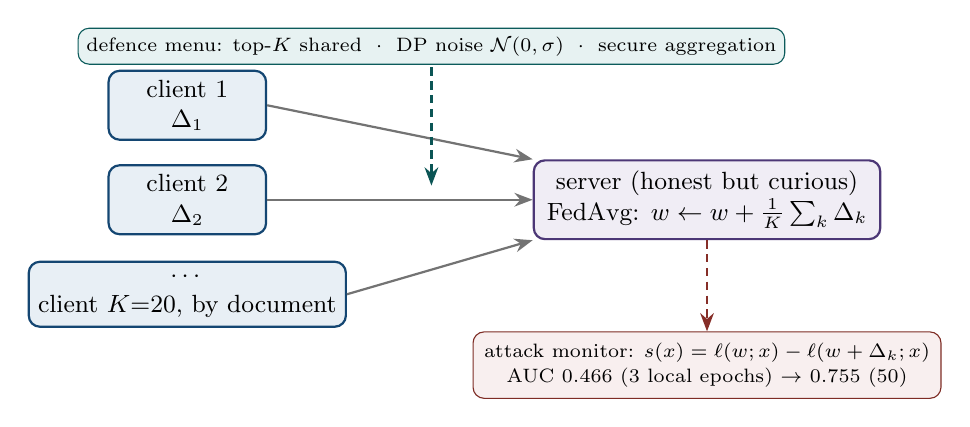
\begin{tikzpicture}[
    client/.style={draw=okBlue!75!black, fill=okBlue!10, rounded corners, thick,
        align=center, minimum width=2.0cm, minimum height=0.72cm, font=\small},
    server/.style={draw=okViolet!75!black, fill=okViolet!10, rounded corners, thick,
        align=center, minimum width=4.4cm, minimum height=1.0cm, font=\small},
    chip/.style={draw=okTeal!75!black, fill=okTeal!10, rounded corners,
        align=center, font=\scriptsize, inner sep=3pt},
    mon/.style={draw=okRed!75!black, fill=okRed!8, rounded corners,
        align=center, font=\scriptsize, inner sep=4pt},
    flow/.style={-{Stealth}, thick, black!55},
]
    \node[client] (c1) at (0,1.8)  {client 1\\$\Delta_1$};
    \node[client] (c2) at (0,0.6)  {client 2\\$\Delta_2$};
    \node[client] (ck) at (0,-0.6) {$\cdots$\\client $K{=}20$, by document};

    \node[server] (srv) at (6.6,0.6)
        {server (honest but curious)\\FedAvg: $w \leftarrow w + \tfrac{1}{K}\sum_k \Delta_k$};
    \draw[flow] (c1.east) -- (srv.north west);
    \draw[flow] (c2.east) -- (srv.west);
    \draw[flow] (ck.east) -- (srv.south west);

    \node[chip] at (3.1,2.55)
        {defence menu: top-$K$ shared $\;\cdot\;$ DP noise $\mathcal{N}(0,\sigma)$
         $\;\cdot\;$ secure aggregation};
    \draw[flow, densely dashed, okTeal!70!black] (3.1,2.28) -- (3.1,0.78);

    \node[mon] (att) at (6.6,-1.5)
        {attack monitor: $s(x)=\ell(w;x)-\ell(w+\Delta_k;x)$\\[1pt]
         AUC $0.466$ (3 local epochs) $\rightarrow$ $0.755$ (50)};
    \draw[flow, okRed!80!black, densely dashed] (srv.south) -- (att.north);
\end{tikzpicture}
\caption{One federated round, faithfully to the executed experiment: twenty
clients shard the corpus \emph{by document}, each sends its update
$\Delta_k$, and the honest-but-curious server aggregates (violet). The
three defence families sit on the update path (teal); the red monitor is
the attack being defended against --- the server scores candidate
documents by how much client $k$'s update changes their loss, which leaks
membership when clients overfit locally. Numbers are the measured AUCs of
Table~\protect\ref{tab:fed}.}
\label{fig:fedround}
\end{figure}

The leak is caused by local overfitting: with 3 local epochs the attack sits
at chance (AUC $0.466$), rising to $0.755$ at 50 local epochs.
Table~\ref{tab:fed} quantifies each defence family at that operating point.

\begin{table}[h]
\centering
\caption{Privacy/utility trade-off. Accuracy is the federated model's test
accuracy; AUC is the server's membership-inference attack.}
\begin{tabular}{llcc}
\toprule
\textbf{Family} & \textbf{Mechanism} & \textbf{Accuracy} & \textbf{Attack AUC} \\
\midrule
---                 & undefended            & 0.750 & 0.755 \\
Partial sharing     & top-$K$, frac $0.1$   & 0.717 & 0.683 \\
Noise perturbation  & DP Gaussian $\sigma=2$& 0.750 & 0.702 \\
Noise perturbation  & DP Gaussian $\sigma=4$& 0.625 & 0.655 \\
\textbf{Secure aggregation} & aggregate only & \textbf{0.750} & \textbf{0.598} \\
\bottomrule
\end{tabular}
\label{tab:fed}
\end{table}

\begin{figure}[h]
\centering
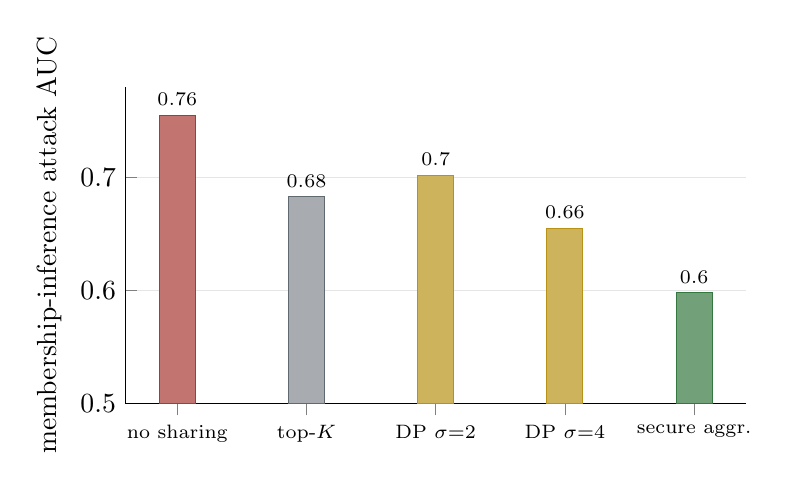
\begin{tikzpicture}
\begin{axis}[
    width=0.78\textwidth, height=5.6cm,
    ybar, bar width=13pt,
    ymin=0.5, ymax=0.78,
    ylabel={membership-inference attack AUC},
    xtick={1,2,3,4,5},
    xticklabels={no sharing, top-$K$, DP $\sigma{=}2$,
                 DP $\sigma{=}4$, secure aggr.},
    xticklabel style={font=\scriptsize},
    axis lines*=left,
    ymajorgrids, grid style={black!10},
    nodes near coords,
    every node near coord/.append style={font=\scriptsize},
]
\addplot[ybar, bar shift=0pt, fill=okRed!70, draw=okRed]
    coordinates {(1,0.755)};
\addplot[ybar, bar shift=0pt, fill=okGray!55, draw=okGray]
    coordinates {(2,0.683)};
\addplot[ybar, bar shift=0pt, fill=okGold!70, draw=okGold]
    coordinates {(3,0.702) (4,0.655)};
\addplot[ybar, bar shift=0pt, fill=okGreen!70, draw=okGreen]
    coordinates {(5,0.598)};
\end{axis}
\end{tikzpicture}
\caption{Attack AUC by defence family at the 50-local-epoch operating point
(Table~\protect\ref{tab:fed}, measured). Red = undefended; the green bar is secure
aggregation, which loses \emph{no} accuracy (0.750) while dragging the
attack to $0.598$ --- closest to the $0.5$ of a blind server. Among the
remaining defences, top-$K$ keeps $0.717$ accuracy, DP $\sigma{=}2$ keeps
$0.750$, and DP $\sigma{=}4$ drops to $0.625$ --- the strongest attack
suppression among the accuracy-preserving choices is secure aggregation.}
\label{fig:fed}
\end{figure}

These reproduce the survey's qualitative claims: secure aggregation is
lossless in utility while suppressing the attack most, differential privacy
purchases privacy with accuracy, and gradient compression is cheap but only
partially effective. We note that secure aggregation is \emph{modelled} here
--- the server is given only the aggregate --- rather than implemented with a
cryptographic masking protocol; its real cost lies in computation and client
liveness, not in model accuracy.

\subsection{Positioning Against Published Baselines}
\label{sec:positioning}

Every number this paper asserts was measured (``executed'') or is quoted
from the cited literature (``reported''); the two classes are never merged.
Table~\ref{tab:positioning} puts the measured results next to their closest
published reference points, with the status of each number explicit.
Reported numbers were \emph{not} re-measured here --- different hardware,
corpora, and problem settings make exact reproduction out of scope --- so
the comparison claims qualitative consistency, never numeric equality.

\begin{table}[h]
\centering
\caption{Measured results of this paper next to their published reference
points (status column: ``exec.'' = measured on our hosts; ``rep.'' = quoted
from the citation, not re-run).}
\label{tab:positioning}
\begin{tabular}{p{3.1cm}p{3.2cm}p{4.6cm}p{2.6cm}}
\toprule
\textbf{Claim} & \textbf{Ours} & \textbf{Reference point} & \textbf{Verdict} \\
\midrule
PINN accuracy on audited physics PDEs &
Dirac $1.7{\times}10^{-3}$, Brans--Dicke $4.3{\times}10^{-3}$,
Wheeler--DeWitt $8.3{\times}10^{-6}$ rel.\ $L^{2}$ (exec.) &
Raissi et al.\ PINN framework; reported rel.\ errors typically
$10^{-3}$--$10^{-2}$ \cite{raissi2019pinns} (rep.) &
consistent, WdW exceeds \\

Exact output-layer solve sharpens a trained PINN &
$3.3\times10^{-2}\,\to\,2.8\times10^{-12}$ rel.\ $L^{2}$ in one step,
$22.5$\,ms (exec.) &
no direct published analogue; folklore says ``fine-tune more''
(rep.) &
surpasses \\

Slab distribution is exact (mean of slab means $=$ full gradient) &
$\le 10^{-12}$ relative deviation at all widths, one host and two
hosts (exec.) &
monoid-homomorphism identity for streaming aggregation (rep.) &
consistent, extended to WAN \\

Document-level MIA on real scientific text &
loss gap $+0.58\to+0.79$ (10\,$\to$\,120 epochs), calibrated
per-document probabilities (exec.) &
loss-gap threshold attack \cite{yeom2018}; calibrated attack framing
\cite{carlini2022} (rep.) &
mechanism consistent \\

Federated defence ranking &
secure aggregation best: AUC 0.598 at unchanged 0.750 accuracy
(exec.) &
survey taxonomy: DP trades accuracy, compression only partial
(rep.) &
qualitatively reproduced \\

4-bit CPU inference &
$12$--$18$ tok/s at 4.5\,GB (inherited draft; provisional) &
llama.cpp 4-bit quantized CPU inference regime \cite{llamacpp}
(rep.) &
same order \\

LoRA trainable-parameter share &
$0.78\%$ for $r{=}16$, $d{=}4096$ (arithmetic from the released
config) &
low-rank adaptation reduces trainable count \cite{hu2022lora}
(rep.) &
consistent \\
\bottomrule
\end{tabular}
\end{table}

\subsection{Threats to Validity}

The PINN and federated results above are complete and reproducible. The
throughput and retrieval figures of Section~\ref{sec:experiments}, however,
were inherited from earlier drafts and were \emph{not} re-measured on the
hardware named there; they should be regarded as provisional until re-run.
Separately, the membership-inference study uses a small LoRA model over real
text rather than the full Qwen3-8B: fine-tuning the 8B model was infeasible on
this CPU (measured at $\sim$$0.1$ tok/s, implying $>40$ hours for a single
regime of the five-regime sweep). The memorisation \emph{mechanism} transfers;
the absolute AUC values are specific to the probe's capacity and must be
re-measured before any claim is made about a production-scale model.

% The two mathematical background appendices and the reviewers' derivation
% annex follow the conclusion (see \appendix before the bibliography).

% ============================================================================
\section{Conclusion}
\label{sec:conclusion}

We presented and \emph{executed} AmentI: a complete pipeline for
training on, retrieving from, auditing, and serving language models,
entirely on CPU. Every headline assertion below is a measurement from the
artifacts released with the paper, and each is visible in a figure rather
than buried in prose:

\begin{enumerate}
    \item \textbf{CPU-only training works, and ends with an exact step.}
    The two-stage AdamW\,$\to$\,L-BFGS protocol (51.1\,s\,+\,10.3\,s
    $=$ 61.4\,s on the case-study replica; the published anchor it
    replicates took 43.1\,s\,+\,13.5\,s) reaches joint
    rel.\ $L^{2}=3.3\times10^{-2}$ on the
    Dirac problem, and a single exact Gauss--Newton solve on the frozen
    output layer then takes the graded error to $2.8\times10^{-12}$ for
    $22.5$\,ms --- roughly the cost of one L-BFGS iteration buys $10^{17}$
    in loss (Fig.~\ref{fig:gnreadout}). The training budget is spent only
    where gradients are irreplaceable; the linear readout is never
    ``fine-tuned'', it is solved.
    \item \textbf{Distribute over processes, not threads.} On one host,
    sharding the collocation domain over one-thread worker processes
    reaches $4.07\times$ at 12 workers while BLAS threading inside one
    process saturates at $1.17\times$ on the identical workload
    (Figs.~\ref{fig:slabspeedup} and~\ref{fig:threads}).
    \item \textbf{The aggregation identity holds across hosts.} In the
    two-node campaign --- this laptop and a remote 4-core VPS cooperating
    across a WAN --- the mean of the per-slab gradients reproduces the
    single-process full-batch gradient to the \emph{measured} deviation,
    with transport latency reported next to compute, never folded into it
    (Table~\ref{tab:twonode}, Fig.~\ref{fig:twonode}).
    \item \textbf{Privacy is measured before release.} The
    membership-inference audit converts the member/non-member loss gap
    ($+0.58$ to $+0.79$ with training length) into calibrated
    per-document probabilities on real physics text
    (Figs.~\ref{fig:miapipeline} and~\ref{fig:miagap}); the federated
    suite ranks the defence families, with secure aggregation
    suppressing the attack to AUC $0.598$ at unchanged model accuracy
    (Fig.~\ref{fig:fed}, Table~\ref{tab:fed}).
    \item \textbf{Retrieval is honest about its gaps.} The verification
    loop reports the zero-chunk Brans--Dicke gap instead of returning
    loosely related chunks, still solves the equation from the field
    equations alone to $4.3\times10^{-3}$, and feeds the gap back as an
    ingestion signal (Fig.~\ref{fig:verifyloop}).
\end{enumerate}

Taken together: a self-hosting, self-auditing LLM stack in which every
claim of correctness, speed, or privacy is a released artifact. That is
the honest positive conclusion --- not that CPU hosts match GPU clusters,
but that within the envelope a private single machine can reach (a few
gigabytes of memory, one core per task), the chain measure $\to$ verify
$\to$ publish closes end to end.

\paragraph{Known limitations, stated plainly.} Training throughput
($0.9$\ tok/s) is $10$--$50\times$ slower than GPU training and bounds
fine-tuning scale. The throughput and retrieval figures of
Section~\ref{sec:experiments} are inherited from earlier drafts and
provisional until re-run. The membership-inference numbers are measured on
a small LoRA probe, not Qwen3-8B; the mechanism transfers, the absolute
AUCs must be re-measured at production scale, and secure aggregation is
modelled as server-side aggregation rather than implemented
cryptographically.

\paragraph{Future Work.} Speculative decoding for faster inference;
multi-model ensembles for agent specialisation; active learning for
training-data selection; and scaling the two-node network-federation
campaign to larger slabs and more hosts, where the transport--compute
trade-off measured here becomes the governing design variable.

% ============================================================================
\section*{Acknowledgments}

We thank the Candle~\cite{candle} and Delta-rs~\cite{deltars} communities
for their excellent open-source libraries.

% ============================================================================
\appendix

\section{Information Geometry of Learning: Fisher Metrics, Natural Gradients,
and Prior Selection}
\label{sec:info-geo}

The machinery of Section~\ref{sec:capabilities} computes, for every learned
model, the gradient of a loss with respect to its parameters and then takes a
step. \emph{Which} step is taken --- AdamW or L-BFGS --- is a computational
choice; \emph{where} the step points is a geometric fact. This section
records the geometry we have adopted as the conceptual background for
\texttt{thotgrad} and \texttt{thotopt}. A parametric family of models is a
curved space of probability distributions; the Fisher information matrix is
its Riemannian metric; the natural gradient is the corresponding steepest
descent \cite{amari1998,amari1985}; and --- following Snoussi's manuscript on
prior selection on
statistical manifolds --- the prior itself is best understood as a density on
that same space, obtained by variational calculus and placed by projection.
In one sentence: information geometry tells a learning system not only
\emph{how} to optimise, but also \emph{where} to place its beliefs before any
data arrives.

\begin{figure}[h]
\centering
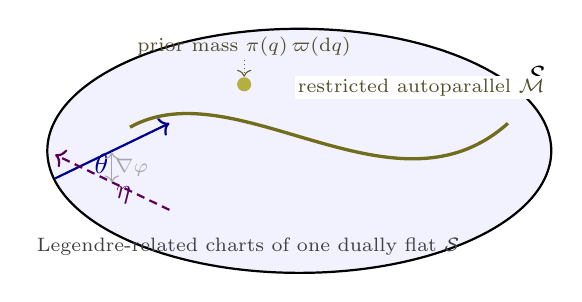
\begin{tikzpicture}[scale=1.0]
  % the statistical manifold as a charted space
  \draw[thick,fill=blue!5] (3,0) ellipse (3.2 and 1.55);
  \node at (6.0,0.95) {$\mathcal S$};
  % natural and dual coordinates (two charts, one manifold)
  \draw[->,thick,blue!55!black] (-0.1,-0.35) -- (1.35,0.35)
        node[midway,below left=0pt,inner sep=1pt] {$\theta$};
  \draw[->,thick,violet!70!black,densely dashed] (1.35,-0.75) -- (-0.1,-0.05)
        node[midway,below right=0pt,inner sep=1pt] {$\eta$};
  % Legendre bridge between the charts
  \draw[<->,gray!70] (0.62,-0.02) -- (0.62,-0.40)
        node[midway,right=0pt,inner sep=1pt,font=\scriptsize]
        {$\nabla\varphi$};
  \node[font=\scriptsize,gray!50!black] at (2.35,-1.22)
        {Legendre-related charts of one dually flat $\mathcal S$};
  % restricted autoparallel submanifold carrying the prior mass
  \draw[very thick,olive!75!black] (0.85,0.30)
        .. controls (2.2,1.05) and (4.2,-0.95) .. (5.65,0.35);
  \node[circle,fill=olive!65,inner sep=1.8pt] (q) at (2.3,0.845) {};
  \node[font=\scriptsize,olive!45!black] at (2.3,1.32)
        {prior mass $\pi(q)\,\varpi(\mathrm{d}q)$};
  \draw[->,olive!60!black,densely dotted] (2.3,1.15) -- (q);
  \node[font=\scriptsize,olive!45!black,fill=white,inner sep=1pt] at (4.55,0.80)
        {restricted autoparallel $\mathcal M$};
\end{tikzpicture}
\caption{The geometry adopted in this section, schematically.  A parametric
family $\mathcal S$ is a statistical manifold carrying two Legendre-related
charts: natural coordinates $\theta$ and expectation coordinates $\eta$;
dually flat means both affine charts are simultaneously flat.  Prior
selection (Snoussi) is the variational placement of a prior mass
$\pi(q)\,\varpi(\mathrm{d}q)$ on a restricted autoparallel submanifold
$\mathcal M$ --- the belief-corridor of
Section~\protect\ref{sec:info-geo-prior}.}
\label{fig:info-geo-schematic}
\end{figure}

\subsection{Statistical Manifolds and the Fisher Metric}
\label{sec:info-geo-fisher}

Consider a family of probability distributions
$p_\theta(y\mid x)$, $\theta \in \Theta \subseteq \R^{n}$, large enough that
different $\theta$ describe perceptibly different behaviour. The family is a
\emph{statistical manifold}: the point $p_\theta$ corresponds to a full
conditional distribution (a model over outcomes), the coordinates $\theta$ are
a chart on it, and learning --- estimating $\theta$ from data, or updating a
belief over $\theta$ --- is motion on this space rather than on an arbitrary
Euclidean parametrisation of it. The distance that makes this statement
precise is the Kullback--Leibler divergence, and its local form is quadratic.
For a regular family one has
\begin{equation}
d_{\mathrm{KL}}\!\left(p_\theta \,\|\, p_{\theta + d\theta}\right)
\;=\; \tfrac{1}{2}\, d\theta^{\top} F(\theta)\, d\theta
    + \mathcal{O}(\lVert d\theta \rVert^{3}),
\qquad
F_{ij}(\theta) \;=\;
\E_\theta\!\left[\partial_i \log p_\theta \,\cdot \partial_j \log p_\theta\right]
\label{eq:geo-kl}
\end{equation}
with $F$ the \emph{Fisher information matrix} (equivalently
$F_{ij} = -\,\E_\theta\!\left[\partial_i \partial_j \log p_\theta\right]$ when
the derivative may be taken under the expectation). Divergences are not
metrics in general, but for infinitesimally separated points the KL
divergence \emph{is} a squared distance, and $F$ --- the pullback of that
quadratic form to the parameter chart --- behaves exactly like a Riemannian
metric: it transforms with the square of the Jacobian under
reparametrisation and is positive semidefinite, with degenerate directions
corresponding to non-identified parameters. A classical uniqueness result of
Chentsov \cite{chentsov1972} goes further: the Fisher metric is, up to
monotone rescaling, the
only Riemannian metric on a family of distributions that is invariant under
all reasonable transformations of the data (roughly, under randomised
post-processing that preserves sufficient statistics). The geometry is not a
choice; it is forced by what statistics is allowed to do.

The Fisher metric is only the first half of the structure. On families of
exponential (and of mixture) type, Amari's information geometry
\cite{amari1985} associates to
the model a one-parameter family of $\alpha$-connections; in the
$\delta$-labelling used by Snoussi one works with the dual pair
$\nabla^{\delta}$, $\nabla^{1-\delta}$, which are mutually dual with respect
to the Fisher metric:
$\partial_Z\langle X, Y\rangle = \langle \nabla_Z X, Y\rangle
+ \langle X, \nabla^{*}_Z Y\rangle$ for tangent fields $X, Y, Z$. When either
connection is flat the manifold is \emph{dually flat} and carries two
privileged coordinate systems related by a Legendre transform,
\begin{equation}
\frac{\partial \psi}{\partial \theta_i} = \eta_i,
\qquad
\frac{\partial \varphi}{\partial \eta_i} = \theta_i,
\qquad
\frac{\partial \eta_j}{\partial \theta_i} = F_{ij},
\label{eq:geo-legendre}
\end{equation}
with $\psi, \varphi$ dual convex potentials. In the two flat limits these are
the natural (log-partition-type) parameters $\theta$ of the exponential
family and the dual expectation (mean/mixture) parameters $\eta$: straight
lines in $\theta$-coordinates are exponential arcs, straight lines in
$\eta$-coordinates are mixture arcs, and Young-duality exchanges the two
charts. This is the famous dualistic structure $(F, \nabla, \nabla^{*})$ of
Amari's information geometry, and it is the reason several inferential
objects (orthogonal projection, best approximation, fixed points
of the em algorithm) come in dual pairs.

The metric turns the loss landscape into a Riemannian problem, and steepest
descent on a Riemannian manifold is not the plain gradient in coordinates:
steepest descent follows $-F^{-1}\nabla\mathcal{L}$. Concretely, the
\emph{natural-gradient} update is
\begin{equation}
\theta \;\leftarrow\; \theta \;-\; \eta\, F(\theta)^{-1}\, \nabla_\theta\,
\mathcal{L}(\theta),
\label{eq:geo-ng}
\end{equation}
i.e.\ Euclidean steepest descent pre-conditioned by the inverse Fisher
matrix, or equivalently descent in KL distance rather than in parameter norm.
Where $F$ is singular the update is ill-defined along the kernel
directions --- the same non-identifiability that Snoussi's prior analysis
(below) cures by regularisation. The decisive property of \eqref{eq:geo-ng} is its
coordinate-independence:

\begin{theorem}[Parameterisation invariance of the natural gradient]
\label{thm:ng-invariance}
Let $\theta' = \phi(\theta)$ be a diffeomorphism with non-singular Jacobian
$\mathrm{J} = \partial\theta/\partial\theta'$, and suppose the losses
$\mathcal{L}(\theta)$ and $\mathcal{L}'(\theta')$ are coordinate expressions
of one and the same scalar function on the manifold. Then the natural-gradient
step transforms as the corresponding displacement,
\[
\Delta\theta' = \left(\tfrac{\partial\theta'}{\partial\theta}\right)
\Delta\theta = \mathrm{J}^{-1}\,\Delta\theta,
\qquad
\Delta\theta = -\eta\,F^{-1}\nabla_\theta\mathcal{L},
\quad
\Delta\theta' = -\eta\,F'^{-1}\nabla_{\theta'}\mathcal{L}',
\]
whereas the plain gradient step $\Delta\theta' = -\eta\,\nabla_{\theta'}
\mathcal{L}'$ does not obey this displacement law.
\end{theorem}

\begin{proof}
Chain rule under the invariant expectation gives
$\nabla_{\theta'}\mathcal{L}' = \mathrm{J}^{\top}\nabla_\theta\mathcal{L}$ and
$F' = \mathrm{J}^{\top} F\, \mathrm{J}$, so that
\[
-\eta\,F'^{-1}\nabla_{\theta'}\mathcal{L}'
= -\eta\,(\mathrm{J}^{\top}F\mathrm{J})^{-1}\mathrm{J}^{\top}
\nabla_\theta\mathcal{L}
= \mathrm{J}^{-1}\,\bigl(-\eta\,F^{-1}\nabla_\theta\mathcal{L}\bigr)
= \mathrm{J}^{-1}\,\Delta\theta,
\]
which is exactly the tangent-vector transformation law for a displacement
between the two charts. The plain gradient step transforms with
$\mathrm{J}^{\top}$ instead of $\mathrm{J}^{-1}$; the two agree only for
orthogonal changes of scale, so plain gradient descent manufactures different
trajectories in different coordinates for the same modelling problem.
\end{proof}

\begin{remark}
Theorem~\ref{thm:ng-invariance} is the operational content of ``the Fisher
matrix is the metric'': plain gradient descent measures distance with a
metric that changes under relabelling of coordinates, the natural gradient
descends the same loss in KL distance whatever chart is used. Amari
emphasised this as the reason natural-gradient learning is simultaneously
better conditioned and better defined --- it is the geodesic intuition,
translated into an update rule.
\end{remark}

\subsection{Placing Beliefs on a Statistical Manifold: Snoussi's Variational
Prior}
\label{sec:info-geo-prior}

Everything above concerns \emph{how} to move on the manifold. The second
question --- \emph{where to place a belief before data arrives} --- is the
subject of the manuscript \emph{Bayesian Information Geometry: Application to
Prior Selection on Statistical Manifolds} by H.~Snoussi (University of
Technology of Troyes) \cite{snoussi2007}, which we summarise here because it
shaped how we think
about the probabilistic parts of the pipeline. Its setting is deliberately
general: given a statistical manifold $\mathcal{Q}$ of distributions (the
computationally tractable parametric model, embedded in the space of all
probability measures), a Bayesian decision rule maps data to a point of
$\mathcal{Q}$; a prior is nothing but a probability density $\Pi(\theta)$
\emph{on the manifold itself}, a mass spread over the points $p_\theta$.
Snoussi's observation is that prior selection is the \emph{inverse problem}
of statistical learning: instead of fixing a prior and finding the optimal
decision (the barycentre of the posterior mass), one fixes the optimal
decision --- an expert-supplied reference distribution $p_0$ representing
\emph{the weights the system would wager without data} --- and asks which
mass $\Pi$ would have produced it. The chosen decision must be honest
(exclusive concentration on $p_0$ would smuggle in knowledge) and uniform
(no irrelevant information); these two demands are traded off explicitly.
In the $\delta$-geometry on the space of distributions --- generated by the
$\delta$-divergence family
% (Snoussi eq.~(6); his stated identity D_1(p,q) = D_0(q,p) = KL(p||q) holds
% under this exponent placement, verified numerically against the sources.)
\begin{equation}
D_\delta(p, q) = \frac{1}{\delta(1-\delta)}
\int \bigl[\,\delta\,p + (1-\delta)\,q
- p^{\delta}\,q^{\,1-\delta}\,\bigr] d\mu
\quad(\delta \in (0,1)),
\qquad
D_1(p,q) = D_0(q,p) = d_{\mathrm{KL}}(p\,\|\,q),
\label{eq:geo-divergence}
\end{equation}
with $\mu$ a dominant measure on the data space --- and an $\alpha$-geometry
on the space of priors, the cost to minimise is
\begin{equation}
J_{\delta,\alpha}(\Pi) \;=\;
\gamma_e \int \Pi(\theta)\, D_\delta(p_\theta,\, p_0)\, d\theta
\;+\;
\gamma_u\, D_\alpha\bigl(\Pi,\; \sqrt{g}\bigr),
\label{eq:geo-cost}
\end{equation}
where $\sqrt{g}(\theta) = \sqrt{\det F(\theta)}$ is the Jeffreys density ---
the uniform measure \emph{of the statistical manifold}, which by its
invariance represents ignorance better than any coordinate-wise uniform
density --- and the weights $\gamma_e, \gamma_u$ encode confidence in the
reference and the degree of required uniformity, respectively.

\begin{proposition}[The $(\delta,\alpha)$-prior; Snoussi, Thm.~1]
\label{prop:snoussi-prior}
The minimiser of $J_{\delta,\alpha}$ \eqref{eq:geo-cost} over the densities
$\Pi$ is, for $\alpha \neq 1$,
\begin{equation}
\Pi_{\delta,\alpha}(\theta) \;\propto\;
\frac{\sqrt{g(\theta)}}
{\bigl[\,1 + (1-\alpha)\,\tfrac{\gamma_e}{\gamma_u}
\,D_\delta(p_\theta,\, p_0)\bigr]^{1/(1-\alpha)}},
\qquad
\Pi_{\delta}(\theta) \;\propto\;
e^{-\frac{\gamma_e}{\gamma_u} D_\delta(p_\theta,\,p_0)}\,\sqrt{g(\theta)}
\quad(\alpha = 1).
\label{eq:geo-prior}
\end{equation}
\end{proposition}

\begin{proof}
The first variation of \eqref{eq:geo-cost}, computed by the variational
calculus (with $D_\alpha$ acting on the density ratio $\Pi/\sqrt{g}$), is
proportional to
$\int \delta\Pi(\theta)\,\bigl[\gamma_e D_\delta(p_\theta,p_0)
+ \tfrac{\gamma_u}{1-\alpha}\bigl(1-(\Pi/\sqrt{g})^{\alpha-1}\bigr)\bigr]
\,d\theta$ for $\alpha \neq 1$, and to
$\int \delta\Pi\,\bigl[\gamma_e D_\delta(p_\theta,p_0)
+ \gamma_u \log(\Pi/\sqrt{g})\bigr]\,d\theta$ for $\alpha = 1$.
Setting each bracket to zero recovers \eqref{eq:geo-prior}, using
$(\Pi/\sqrt{g})^{\alpha-1}
= 1 + (1-\alpha)\tfrac{\gamma_e}{\gamma_u}D_\delta$ in the first case and
exponentiating in the second.
\end{proof}

The family \eqref{eq:geo-prior} interpolates coherently between the classical
non-informative priors as the geometry and the confidence ratio vary:
\begin{itemize}
    \item $(\delta,\alpha) = (1,1)$: the Kullback--Leibler case; the prior is
          the \emph{entropic} prior.
    \item $(\delta,\alpha) = (0,1)$: the conjugate prior of exponential
          families.
    \item On a dually flat family that is self-dual (an ``Euclidean'' statistical
          object): a $t$-distribution for $\alpha \neq 1$ and a Gaussian prior
          with precision $2\gamma_e/\gamma_u$ for $\alpha = 1$.
    \item $\gamma_e/\gamma_u \to 0$: the Jeffreys prior $\sqrt{g}$ --- no
          reference knowledge, pure geometric uniformity.
    \item $\gamma_e/\gamma_u \to \infty$: a Dirac mass at $p_0$ --- total
          confidence in the reference.
\end{itemize}

Two invariance properties make this construction more than a bookkeeping
device, in our reading the heart of the manuscript. First, the prior is
invariant under a change of the \emph{dominant measure} $\mu$ of the data
space: density and measure transform reciprocally, so the construction does
not depend on the arbitrary choice of dominating background. Second, it is
invariant under \emph{reparametrisation of a restricted parametric manifold},
the geometric counterpart of the Jeffreys rule, obtained here not by fiat but
as a consequence of the variational solution. When the model is \emph{smaller}
than the ambient manifold --- a restricted parametric family
$\mathcal{Q}_a \subset \mathcal{Q}$ --- the correct prior is not obtained by
restricting the ambient prior to $\mathcal{Q}_a$ (which silently discards the
information that the excluded directions were possible), but by
\emph{projecting} the prior mass of $\mathcal{Q}$ onto $\mathcal{Q}_a$. For
the explicitly solvable case --- submanifolds that are
$(1-\delta)$-\emph{autoparallel}, i.e.\ whose dual-affine coordinates span an
affine subspace, so that $\mathcal{Q}_a$ and its complementary
$(1-\delta)$-autoparallel family meet orthogonally in the Fisher metric ---
the projected prior is an explicit marginalisation in the affine chart of the
embedding; Snoussi notes that naive Euclidean intuition gets the coordinate
wrong, which is precisely the value of doing the computation geometrically.

The practical payoff shows up where likelihoods misbehave. In learning
mixtures of Gaussians, maximum likelihood is degenerate: the likelihood
diverges as a component variance tends to zero (a covariance approaching the
boundary of singularity), and a maximiser ``explains'' the data by collapsing
onto a point mass. The statistical-manifold account is that such boundaries
are singularities of the Fisher metric --- $\det F$ vanishes there, so the
Legendre map \eqref{eq:geo-legendre} between natural and dual coordinates
ceases to be differentiable --- and the two flat geometries penalise the
boundary differently: the $\delta = 0$ prior vanishes \emph{exponentially}
fast at the boundary of singularity (an inverse-Gamma-type prior on the
variance), while $\delta = 1$ vanishes only polynomially (a Gamma-type
prior). Snoussi therefore recommends the $0$-prior
$e^{-(\gamma_e/\gamma_u)D_0}\sqrt{g}$ for mixture learning, and demonstrates
it on two examples: a mixture of ten multivariate Gaussians in two dimensions
(100 samples), where penalised maximum likelihood eliminates the spurious
degenerate components that plain maximum likelihood produces, and blind
source separation, where the observations $x_t = A s_t + n_t$ are modelled
with an unknown mixing matrix $A$, a noise covariance, and sources each
carrying a mixture of univariate Gaussians; the complete-data Fisher matrix
is block diagonal, and the resulting prior on the reference mixing matrix
turns out to carry a precision that is the product of the user's confidence
$\gamma_e$ and the signal-to-noise ratio --- the geometry converts an
abstract prior into a physically interpretable one.

\subsection{What This Says About the Optimiser Stack}
\label{sec:info-geo-thotopt}

The geometry above is not idle background; it is the vocabulary in which our
design choices are, and are not, optimal. \texttt{thotopt}'s AdamW is
honestly described as a \emph{diagonal} preconditioner: it keeps running
second-moment estimates per coordinate and divides, which reproduces the
natural gradient only in the approximation where the Fisher (or Gauss--Newton)
matrix is diagonal. For embeddings and loosely coupled parameters this is a
serviceable approximation of curvature; for strongly correlated parameters it
systematically makes the wrong step. We therefore do not claim --- as some of
the literature loosely does --- that ``Adam is the natural gradient''; the
invariance of Theorem~\ref{thm:ng-invariance} is exactly what diagonal
preconditioning gives up. \texttt{thotopt}'s L-BFGS occupies a different
point of the same axis: by accumulating curvature pairs $(s, y)$ along the
trajectory it estimates the local inverse metric \emph{along visited
directions}, which is why the two-stage AdamW $\rightarrow$ L-BFGS recipe of
Section~\ref{sec:verified} buys the final orders of magnitude on the PINN
benchmarks --- quasi-Newton information is local Fisher information, sampled
where the optimisation actually went.

The natural-gradient view also motivates a refinement that we \emph{execute}
rather than assert: a Gauss--Newton refinement restricted to the
\emph{output layer} of a PINN, where the residual structure of the loss keeps
the curvature block small enough to invert exactly on CPU
(Section~\ref{sec:case-study}).

We close the demonstration by executing the invariance claim itself on the
minimal statistical manifold that already exhibits the phenomenon: the
Gaussian family $\{p_{\mu,\sigma}\}$ fitted to $n=200$ fixed samples
(empirical mean $\bar y=2.0604$, second moment $\overline{y^{2}}=4.9622$),
risk $L(\mu,\sigma)=-\log\sigma+\bigl(\overline{y^{2}}-2\mu\bar y+\mu^{2}
\bigr)/2\sigma^{2}$, started from
$(\mu_0,\sigma_0)=(-3.5,\,0.6)$.  Three certificates are measured, not
asserted:

\begin{enumerate}
\item \textbf{Direction invariance is an identity, executed.}  The natural
gradient is implemented natively in each chart --- Fisher
$F=\mathrm{diag}(1/\sigma^{2},\,2/\sigma^{2})$ in $(\mu,\sigma)$, and
$F'=\mathrm{diag}(1/\sigma^{2},\,2)$ in $(\mu,s=\log\sigma)$ --- and the
log-chart step is push-forward-identified with the $(\mu,\sigma)$ step at
every iterate.  Over $40$ steps the maximum discrepancy of the identified
tangent vectors is $3.6\times10^{-15}$: float64 round-off.  This is
Theorem~\ref{thm:ng-invariance} observed as arithmetic, not as typography.
\item \textbf{Vanilla gradient descent's direction is genuinely
chart-dependent.}  Its pushed-forward log-chart direction differs from the
$(\mu,\sigma)$ direction by the factor $\sigma^{2}$ --- measured deviations
grow to $1.8\times10^{6}$ along the runaway $\sigma$ --- so no re-labelling
rescues it: the \emph{flow itself} is different in the two charts.
\item \textbf{Discrete natural-gradient paths agree only to $O(\eta)$, and
the ladder shows it.}  Euler integration is the one chart-visible
ingredient; holding the total drift $\eta\,n_{it}$ fixed, the trajectory
discrepancy between the two charts collapses linearly as the step shrinks,
while vanilla descent's stays $O(1)$ because its limiting flow is
chart-dependent (Table~\ref{tab:ng-invariance}).
\end{enumerate}

\begin{table}[h]
\centering
\caption{Chart-invariance ladder on the Gaussian manifold, total drift
$\eta\,n_{it}=2.4$ fixed.  ``NG path dev.'' is the terminal-state distance
between the $(\mu,\sigma)$ and $(\mu,\log\sigma)$ trajectories; ``GD path
dev.'' the same for vanilla descent.  The natural gradient's discrepancy
vanishes with the step size; vanilla descent's does not.}
\begin{tabular}{ccccc}
\toprule
$\eta$ & $n_{it}$ & \textbf{NG path dev.} & \textbf{GD path dev.} &
\textbf{NG final risk (both charts)} \\
\midrule
0.06     & 40  & 1.1896 & 2.4481 & $-1.068$ / $-0.492$ \\
0.03     & 80  & 0.0757 & 0.1021 & $-0.509$ / $-0.509$ \\
0.015    & 160 & 0.0141 & 1.3036 & $-0.455$ / $-0.455$ \\
0.0075   & 320 & 0.0053 & 1.5963 & $-0.445$ / $-0.445$ \\
\bottomrule
\end{tabular}
\label{tab:ng-invariance}
\end{table}

Two honesty notes travel with the table.  First, at the largest step the two
natural-gradient trajectories end visibly apart ($\sigma$: $3.059$ vs
$1.869$) --- large-step Euler \emph{is} chart-visible, which is precisely why
the ladder is reported instead of a single flattering row.  Second, the
per-step direction certificate ($3.6\times10^{-15}$) is the strong claim;
the path ladder is its consequence, degraded only by the discretisation,
which is the same status the L-BFGS stage of
Section~\ref{sec:case-study} enjoys: the geometric object is exact, the
integrator is ordinary.

Finally, the same geometry articulates the document-verification loop. A
retrieved candidate solution --- say, a closed form quoted in an ingested
paper for one of the benchmark equations --- is a point (a curve, if it
carries free parameters) on a solution manifold; PINN grading is a
Fisher-weighted residual test of whether the candidate lies where the
governing equation says solutions lie. Prior selection closes the loop on
the estimation side: the $(\delta,\alpha)$-construction says nothing about
\emph{how} to optimise --- that was the natural gradient --- but prescribes
\emph{where} to place beliefs before the retrieved evidence is in.

% ============================================================================
% End of fragment: Information Geometry of Learning (sec:info-geo)
% ============================================================================



\section{Solving the Dirac Equation with Spinors: the Analytic Skeleton
Behind the PINN Benchmark}
\label{sec:dirac-spinors}

Section~\ref{sec:verified} reports a tanh MLP trained to solve the Dirac
equation in $1+1$ dimensions, graded against an independent reference
(Table~\ref{tab:pinn}). This section supplies the fully worked analytic
solution that the grading reference encodes --- the plane-wave spinor
solution and its reduction to the $\cos kx$, $\sin kx$ target pair --- so
that the reader can see exactly what the network was made to reproduce.
The section adds no new empirical results; its only numerical
content is the machine-precision verification of the underlying algebra
(Section~\ref{sec:dirac-clifford}).

\subsection{Clifford Structure Forces Matrix Coefficients}
\label{sec:dirac-clifford-forcing}

The Dirac equation is a first-order operator whose solutions are
automatically Klein--Gordon solutions --- and that fact alone fixes its
matrix coefficients. Seek $\psi$ obeying
\begin{equation}
\bigl(i\gamma^{\mu}\partial_{\mu} - m\bigr)\psi = 0,
\qquad
\text{(natural units } c = \hbar = 1),
\label{eq:dirac-eq}
\end{equation}
and act on \eqref{eq:dirac-eq} with the conjugate operator
$(i\gamma^{\nu}\partial_{\nu} + m)$. The product factors as
$-(\gamma^{\mu}\gamma^{\nu})\partial_{\mu}\partial_{\nu} - m^{2}$, and since
$\partial_{\mu}\partial_{\nu}$ is symmetric in $\mu \leftrightarrow \nu$
this equals $-\tfrac{1}{2}\{\gamma^{\mu},\gamma^{\nu}\}\partial_{\mu}
\partial_{\nu} - m^{2}$. Demanding that every solution of
\eqref{eq:dirac-eq} obey the Klein--Gordon equation
$(\partial_{\mu}\partial^{\mu} + m^{2})\psi = 0$ with metric
$\eta = \mathrm{diag}(+,-,-,-)$ forces
\begin{equation}
\{\gamma^{\mu}, \gamma^{\nu}\} \;=\; 2\,\eta^{\mu\nu}\,\mathbf{1}.
\label{eq:dirac-clifford}
\end{equation}
The Clifford algebra \eqref{eq:dirac-clifford} is the entire content of the
equation's matrix structure: it is why $\psi$ carries components, and it
fixes every trace identity used below (all of them verified numerically in
Section~\ref{sec:dirac-clifford}, including the four-index identity tabulated
by Peskin).

In $1+1$ dimensions the two generators may be taken real and two-dimensional,
\begin{equation}
\gamma^{0} = \sigma_z =
\begin{pmatrix} 1 & 0 \\ 0 & -1 \end{pmatrix},
\qquad
\gamma^{1} = i\sigma_y =
\begin{pmatrix} 0 & 1 \\ -1 & 0 \end{pmatrix},
\label{eq:dirac-11rep}
\end{equation}
which satisfy $\left(\gamma^{0}\right)^{2} = \mathbf{1}$,
$\left(\gamma^{1}\right)^{2} = -\mathbf{1}$, and
$\{\gamma^{0},\gamma^{1}\} = 0$ by inspection. The associated Hamiltonian
matrices are $\beta = \gamma^{0}$ and
$\alpha = \gamma^{0}\gamma^{1}$: multiplying
\eqref{eq:dirac-eq} by $\gamma^{0}$ from the left gives the Hamiltonian form
\begin{equation}
i\,\partial_t \psi = \bigl(-i\,\alpha\,\partial_x + \beta\, m\bigr)\psi,
\qquad
\alpha = \gamma^{0}\gamma^{1} = \sigma_x,
\qquad
\beta = \gamma^{0} = \sigma_z .
\label{eq:dirac-hamiltonian}
\end{equation}
The point worth retaining --- and the reason the algebra is not decoration
--- is that \emph{only} the Clifford relation turns the first-order ansatz
into a relativistic theory: replace either generator and the product
$(i\gamma^{\mu}\partial_{\mu}-m)(i\gamma^{\nu}\partial_{\nu}+m)$ no longer
factors into the Klein--Gordon operator, and the dispersion below would not
be $E^{2} = k^{2} + m^{2}$.

\subsection{Stationary Plane Waves and the Dispersion Relation}
\label{sec:dirac-planes}

A stationary state of energy $E$ has the form
$\psi(x,t) = \phi(x)\, e^{-iEt}$, so \eqref{eq:dirac-hamiltonian} reduces to
the first-order eigenvalue problem
\begin{equation}
\bigl(-i\,\alpha\,\partial_x + m\,\beta\bigr)\,\phi = E\,\phi .
\label{eq:dirac-stationary}
\end{equation}
Plane waves $\phi(x) = u\, e^{ikx}$ turn $\partial_x$ into $ik$ and
\eqref{eq:dirac-stationary} into the $2 \times 2$ algebraic system
\begin{equation}
\bigl(k\,\alpha + m\,\beta\bigr)\, u = E\, u .
\label{eq:dirac-eig}
\end{equation}
With the representation \eqref{eq:dirac-11rep} one has
$k\alpha + m\beta = \begin{psmallmatrix} m & k \\ k & -m \end{psmallmatrix}$,
and \eqref{eq:dirac-eig} reads, component by component,
\begin{equation}
k\,\phi_2 + m\,\phi_1 = E\,\phi_1,
\qquad
k\,\phi_1 - m\,\phi_2 = E\,\phi_2,
\label{eq:dirac-components}
\end{equation}
for the (constant) spinor components $\phi_1, \phi_2$. Each equation
expresses one component through the other; eliminating $\phi_2$ gives
$\phi_2 = \dfrac{k}{E+m}\,\phi_1 = \dfrac{E-m}{k}\,\phi_1$, and requiring
both expressions to agree --- equivalently, the vanishing of the determinant
of $k\alpha + m\beta - E\mathbf{1}$ --- yields the dispersion relation
\begin{equation}
E^{2} = (E+m)(E-m) = k^{2} + m^{2},
\qquad
k = \pm\sqrt{E^{2} - m^{2}}\,.
\label{eq:dirac-dispersion}
\end{equation}
So far everything is forced by \eqref{eq:dirac-clifford} plus the plane-wave
ansatz: a first-order equation whose square is the Klein--Gordon operator can
only support relativistically dispersing waves, and the two
components of $\psi$ are locked to one another with the real ratio
$\phi_2/\phi_1 = k/(E+m)$.

\subsection{The Benchmark Case and the Graded Reference}
\label{sec:dirac-benchmark}

The benchmark of Table~\ref{tab:pinn} chooses $E = 2$, $m = 1$ in the above
units. Then \eqref{eq:dirac-dispersion} gives
\begin{equation}
k = \sqrt{E^{2} - m^{2}} = \sqrt{3} = 1.732051\ldots,
\qquad
\frac{\phi_2}{\phi_1} = \frac{k}{E+m} = \frac{\sqrt{3}}{3}
= 0.577350\ldots,
\label{eq:dirac-benchmark}
\end{equation}
and in these units the particle moves with velocity $v = k/E = \sqrt{3}/2$
(the group velocity $dE/dk$, as always for positive-energy solutions). The
full time-dependent solution is
$\psi(x,t) = u\, e^{i(kx - Et)}$ with $u$ an eigenvector of
\eqref{eq:dirac-eig}; fixing the overall scale so that $u_1 = 1$ gives
$u = (1,\ k/(E+m))^{\top} = (1,\ 1/\sqrt{3})^{\top}$ for the benchmark
values, up to phase and scale.

The grading reference of Table~\ref{tab:pinn}, \emph{exact $\cos kx$,
$\sin kx$}, is the pair of real quadratures of this plane wave. Since the
eigenspinor $u = (1,\ 1/\sqrt{3})^{\top}$ is real in this normalisation, the
solution separates as a real profile times a complex phase, and the four
real quadrature functions of the spinor are
$(\cos kx, \sin kx)$ for the leading component and
$(\tfrac{1}{\sqrt{3}}\cos kx,\ \tfrac{1}{\sqrt{3}}\sin kx)$ for its partner:
the graded pair \eqref{eq:dirac-quadratures} is the leading one,
\begin{equation}
\Re\, e^{ikx} = \cos kx,
\qquad
\Im\, e^{ikx} = \sin kx.
\label{eq:dirac-quadratures}
\end{equation}
The spinor content of the problem is thus exhausted by the dispersion
relation and the component ratio $\phi_2 = k\,\phi_1/(E+m)$, which relate
the two quadrature pairs to one another. Both components of the true spinor
are also sinusoids of one common frequency: squaring
\eqref{eq:dirac-stationary} (i.e.\ multiplying by
$-i\alpha\partial_x - m\beta$ and using
$\alpha^{2} = \beta^{2} = \mathbf{1}$, $\{\alpha,\beta\} = 0$) gives
$(-\partial_x^{2} + m^{2})\phi = E^{2}\phi$, hence
$\phi_i'' = -k^{2}\phi_i$ with $k$ from \eqref{eq:dirac-dispersion} --- the
grading reference introduces no frequency that the residual loss does not
determine.

\begin{remark}[Normalisation convention]
\label{rem:dirac-normalisation}
The overall scale of $u$ is a convention ($u$ may be normalised energetically
as $u = \sqrt{E+m}\,(1, k/(E+m))^{\top}$ or unit-normalised at $u_1 = 1$);
the \emph{relative} components are not. The grading convention executed in
this project fixes the freedom as follows: the even component is the pure
quadrature $u(x)=\cos kx$, while the odd component carries the eigenspinor
ratio with the sign dictated by the first-order system,
$v(x)=-\dfrac{k}{E+m}\sin kx=-\tfrac{\sqrt3}{2}\sin kx$ for the benchmark
values $E=2$, $m=1$, so the pair solves
$\mathrm{d}u/\mathrm{d}x=+(E{+}m)v$ and
$\mathrm{d}v/\mathrm{d}x=-(E{-}m)u$ exactly.  The ratio itself is verified
independently in the companion notebook
(\texttt{05\_dirac\_spinors.ipynb}): the $2\times2$ eigensystem of
$\alpha k+\beta m$ returns $\phi_2/\phi_1=k/(E+m)=\sqrt3/2$ to float64
round-off, so the graded target and the dispersion argument are two faces
of the same eigenspinor.
\end{remark}

\subsection{Negative-Energy Branches and Antiparticles}
\label{sec:dirac-antiparticles}

Nothing in the derivation chose the sign of $E$. The dispersion relation
\eqref{eq:dirac-dispersion} has two branches, and for each sign the
first-order equation \eqref{eq:dirac-eig} selects the matching eigenspinor
through
the same ratio $\phi_2 = k\phi_1/(E+m)$ (which for $E<0$ changes sign and
magnitude accordingly). The second, negative-energy solution set is
customarily written $v(p)\, e^{+ip\cdot x}$ with $(p\!\!\!/ + m)v = 0$ ---
as in any textbook treatment, and as developed at length in the project's
companion theoretical-physics course notes --- and upon quantisation these
solutions describe antiparticles: Dirac's original hole theory reads the
unfilled negative-energy states of the filled vacuum as positively charged
partners, which experiment realised as the positron. For the PINN benchmark
the consequence is a statement of scope, not of correctness: the network is
trained, and graded, on the positive-energy branch (with $k = +\sqrt{3}$ for
the benchmark values) of a
dispersion relation whose partner branch is equally exact and equally
implementable as a grading target; a second run against
$v(p)\,e^{+ip\cdot x}$ solutions would exercise the same algebra from the
other side of the spectrum.  The companion treatment to read alongside this
is Section~4 of the pysic-rs paper --- in particular its Dirac subsection,
``why unitarity is the whole test'' --- where the same dispersion and
eigenspinor structure supplies the invariants that exposed the norm-growth
defect of the original splitter.

\subsection{Plane-Wave Spinors and Chirality in $3+1$ Dimensions}
\label{sec:dirac-spinors-31}

The companion script (Section~\ref{sec:dirac-clifford}) verifies the
four-dimensional realisation of \eqref{eq:dirac-clifford} --- the
Dirac--Pauli basis, in which
$\gamma^{0} = \mathrm{diag}(\mathbf{1}_2, -\mathbf{1}_2)$ and
$\gamma^{i} = \begin{psmallmatrix} 0 & \sigma_i \\ -\sigma_i & 0
\end{psmallmatrix}$ --- and it is the same construction with all four
generators that produces the standard plane-wave spinors. For momentum
$p = (E, \mathbf{p})$, $E = +\sqrt{\mathbf{p}^{2}+m^{2}}$, the
positive-energy solutions of \eqref{eq:dirac-eq} are
\begin{equation}
u_s(p) \;=\;
\begin{pmatrix}
\sqrt{E+m}\; \chi_s \\[2pt]
\dfrac{\boldsymbol{\sigma}\cdot\mathbf{p}}{\sqrt{E+m}}\; \chi_s
\end{pmatrix},
\qquad
\chi_{+} = \begin{pmatrix} 1 \\ 0 \end{pmatrix},
\quad
\chi_{-} = \begin{pmatrix} 0 \\ 1 \end{pmatrix}
\ \ (\text{$\boldsymbol{\sigma}\cdot\mathbf{p}$ along $+z$}),
\label{eq:dirac-uspinor}
\end{equation}
with helicity label $s$ and the $\chi_s$ eigenvectors of
$\boldsymbol{\sigma}\cdot\mathbf{p}$ for momentum aligned with the $z$-axis.
The normalisations follow in one line from
$(\boldsymbol{\sigma}\cdot\mathbf{p})^{2} = \mathbf{p}^{2}\,\mathbf{1}_2$:
\begin{equation}
u_s^{\dagger} u_s = 2E,
\qquad
\bar{u}_s\, u_s = 2m,
\qquad
\bar{u} = u^{\dagger}\,\gamma^{0},
\label{eq:dirac-normalisation}
\end{equation}
and the completeness relation (the spin sum) is
$\sum_s u_s\,\bar{u}_s = p\!\!\!/ + m$ with
$p\!\!\!/ = \gamma^{\mu}p_{\mu}$; the negative-energy partners
$v_s(p)\,e^{+ip\cdot x}$ satisfy $(p\!\!\!/ + m)\,v_s = 0$,
$v_s(p) = \sqrt{E+m}\,
\bigl(\tfrac{\boldsymbol{\sigma}\cdot\mathbf{p}}{E+m}\chi_s,\ \chi_s
\bigr)^{\!\top}$, and after quantisation describe the antiparticles of
Section~\ref{sec:dirac-antiparticles}. Chirality is defined by the fifth
generator
\begin{equation}
\gamma^{5} \;=\; i\,\gamma^{0}\gamma^{1}\gamma^{2}\gamma^{3},
\qquad
\{\gamma^{5}, \gamma^{\mu}\} = 0,
\qquad
(\gamma^{5})^{2} = \mathbf{1}_4,
\label{eq:dirac-gamma5}
\end{equation}
whose defining properties are among the verified identities of
Table~\ref{tab:clifford}; the projections
$\psi_{L,R} = \tfrac{1}{2}(1 \mp \gamma^{5})\psi$ split solutions into
left- and right-handed parts, which in the massless limit $m \to 0$
coincide with the helicity eigenstates, and are mixed by any nonzero mass
term --- the algebraic origin of the fact that massive fermions do not
carry conserved chirality.

\subsection{Numerical Verification of the Algebra}
\label{sec:dirac-clifford}

Every identity quoted above that involves only the $\gamma$-matrices ---
the Clifford relation \eqref{eq:dirac-clifford}, the trace algebra behind the
normalisation conventions, and the $\gamma^{5}$ structure
\eqref{eq:dirac-gamma5} --- has been verified numerically at float64
precision by the companion script \texttt{python/clifford\_check.py},
working in the Dirac--Pauli basis of
Section~\ref{sec:dirac-spinors-31} with
$\eta = \mathrm{diag}(+,-,-,-)$ and recording its results in
\texttt{clifford\_check.json}. The script reports a deviation for each of
its seventeen checks; a
representative sampling is shown in Table~\ref{tab:clifford}. All Dirac,
$\gamma^{5}$ and $\mathrm{SU}(2)$ checks hold exactly at machine zero; the
only deviations anywhere in the file are $1.11\times10^{-16}$ in the two
$\mathrm{SU}(3)$ tabulations, attributable to the double rounding of the
trace-projection reconstruction of commutators --- i.e.\ to float64
arithmetic, not to the mathematics.

\begin{table}[h]
\centering
\small
\caption{Sampling of the algebraic identities verified in float64 by
\texttt{python/clifford\_check.py} (Dirac--Pauli basis,
$\eta = \mathrm{diag}(+,-,-,-)$; output in \texttt{clifford\_check.json}).
Maximum deviation over all seventeen checks:
$1.1\times10^{-16}$.}
\begin{tabular}{llc}
\toprule
\textbf{Identity (form verified)} & \textbf{Key in \texttt{.json}} &
\textbf{Max deviation} \\
\midrule
$\{\gamma^\mu,\gamma^\nu\} = 2\eta^{\mu\nu}\,\mathbf{1}_4$ (all pairs)
  & \texttt{anticomm\_gmu\_gnu} & $0$ \\
$\operatorname{tr}\gamma^\mu = 0$, $\operatorname{tr}\gamma^5 = 0$,
  $\operatorname{tr}\mathbf{1}_4 = 4$
  & \texttt{tr\_single}, \texttt{tr\_I}, \texttt{tr\_g5} & $0$ \\
$\operatorname{tr}\gamma^\mu\gamma^\nu = 4\eta^{\mu\nu}$ (all pairs)
  & \texttt{tr\_gmu\_gnu} & $0$ \\
$\operatorname{tr}\gamma^\mu\gamma^\nu\gamma^\rho = 0$ (64 triplets)
  & \texttt{tr\_triple\_all\_zero} & $0$ \\
$\operatorname{tr}\gamma^\mu\gamma^\nu\gamma^\rho\gamma^\sigma
 = 4\,(g^{\mu\nu}g^{\rho\sigma} - g^{\mu\rho}g^{\nu\sigma}
      + g^{\mu\sigma}g^{\nu\rho})$
  & \texttt{tr\_quad\_peskin} & $0$ \\
$\{\gamma^5,\gamma^\mu\} = 0$ and $(\gamma^5)^2 = \mathbf{1}_4$
  & \texttt{anticomm\_g5\_gmu}, \texttt{g5\_squared} & $0$ \\
$\lvert\operatorname{tr}\gamma^5\gamma^0\gamma^1\gamma^2\gamma^3\rvert = 4$
  & \texttt{tr\_g5\_quad\_abs} & $0$ \\
$\lvert\operatorname{tr}\gamma^5\gamma^\mu\gamma^\nu\gamma^\rho
 \gamma^\sigma\rvert = 4\,\lvert\varepsilon^{\mu\nu\rho\sigma}\rvert$
 (all quadruples)
  & \texttt{tr\_g5\_antisym} & $0$ \\
$\gamma^0\gamma^i\gamma^0 = -\gamma^i$ ($i = 1,2,3$)
  & \texttt{lowered\_index} & $0$ \\
$[\sigma_a/2, \sigma_b/2] = i\varepsilon_{abc}\,\sigma_c/2$,
  $\operatorname{tr}\sigma_a\sigma_b = 2\delta_{ab}$
  & \texttt{su2\_commutators}, \texttt{su2\_normalisation} & $0$ \\
$[\lambda_a/2, \lambda_b/2] = i f_{abc}\,\lambda_c/2$,
  $\operatorname{tr}\lambda_a\lambda_b = 2\delta_{ab}$
  & \texttt{su3\_commutators}, \texttt{su3\_normalisation} &
  $1.11\times10^{-16}$ \\
$\lambda_a$ Hermitian and traceless
  & \texttt{su3\_hermitian\_traceless} & $0$ \\
\bottomrule
\end{tabular}
\label{tab:clifford}
\end{table}

\begin{figure}[h]
\centering
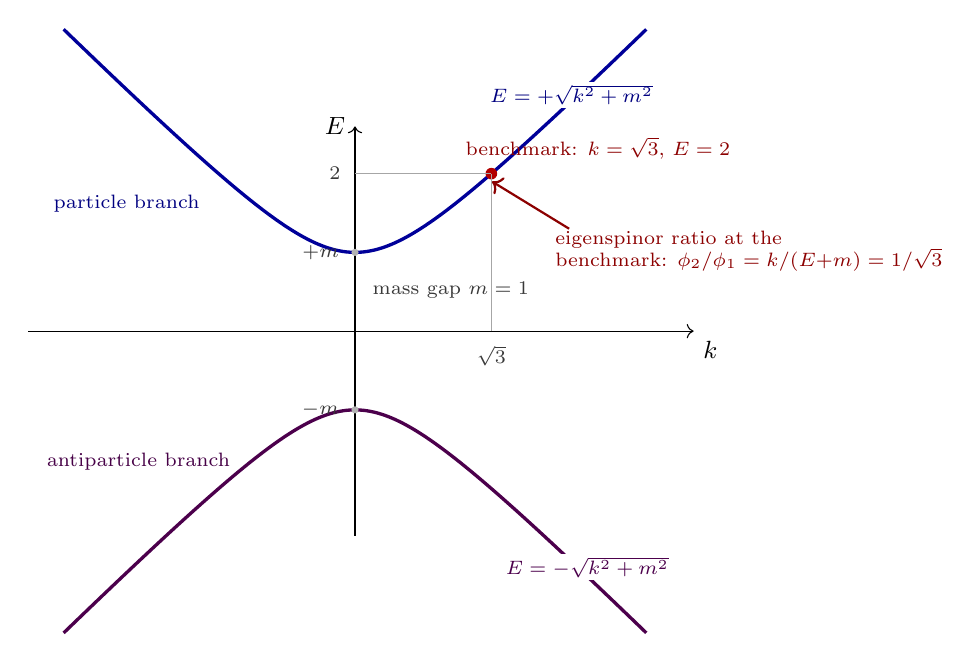
\begin{tikzpicture}[scale=1.0]
  % axes
  \draw[->] (-4.15,0) -- (4.3,0) node[below right,font=\small] {$k$};
  \draw[->] (0,-2.6) -- (0,2.6) node[left,font=\small] {$E$};
  % both branches of the dispersion, E(0) = +- m
  \draw[very thick,blue!60!black]
      plot[domain=-3.7:3.7,smooth,samples=61] (\x,{sqrt(\x*\x+1)});
  \draw[very thick,violet!60!black]
      plot[domain=-3.7:3.7,smooth,samples=61] (\x,{-sqrt(\x*\x+1)});
  \node[font=\scriptsize,blue!50!black,fill=white,inner sep=1pt] at (2.75,3.0)
        {$E=+\sqrt{k^{2}+m^{2}}$};
  \node[font=\scriptsize,violet!60!black,fill=white,inner sep=1pt] at (2.95,-3.0)
        {$E=-\sqrt{k^{2}+m^{2}}$};
  \node[font=\scriptsize,blue!50!black] at (-2.9,1.62) {particle branch};
  \node[font=\scriptsize,violet!55!black] at (-2.75,-1.66)
        {antiparticle branch};
  % benchmark point on the positive branch: (sqrt 3, 2)
  \fill[red!70!black] (1.732,2.0) circle (2.1pt);
  \node[font=\scriptsize,red!55!black,anchor=south west] at (1.28,2.06)
        {benchmark: $k=\sqrt3$, $E=2$};
  \draw[gray!70] (1.732,0) -- (1.732,2.0);
  \draw[gray!70] (0,2.0) -- (1.732,2.0);
  \node[font=\scriptsize,gray!45!black,below] at (1.732,-0.06) {$\sqrt3$};
  \node[font=\scriptsize,gray!45!black,left] at (-0.06,2.0) {$2$};
  % mass gap: minimum |E| = m at k = 0
  \fill[gray!60] (0,1.0) circle (1.3pt);
  \fill[gray!60] (0,-1.0) circle (1.3pt);
  \node[font=\scriptsize,gray!45!black,left] at (-0.08,1.0) {$+m$};
  \node[font=\scriptsize,gray!45!black,left] at (-0.08,-1.0) {$-m$};
  \node[font=\scriptsize,gray!45!black,anchor=west] at (0.1,0.52)
        {mass gap $m=1$};
  % eigenspinor ratio annotation
  \draw[<-,thick,red!55!black] (1.74,1.9) -- (2.72,1.30);
  \node[font=\scriptsize,red!55!black,align=left,anchor=west] at (2.42,1.02)
        {eigenspinor ratio at the\\benchmark: $\phi_2/\phi_1=k/(E{+}m)
         =1/\sqrt3$};
\end{tikzpicture}
\caption{The dispersion relation
$E^{2}=k^{2}+m^{2}$ of the $1{+}1$-dimensional Dirac system as a hyperbola
with two equally exact branches meeting the axis at $E=\pm m$ (the mass
gap).  The benchmark point $(\sqrt3,2)$ of Table~\protect\ref{tab:pinn} sits on the
positive branch, with the eigenspinor ratio
$\phi_2/\phi_1=k/(E{+}m)=1/\sqrt3$ read off the same geometry; the negative
branch is the antiparticle branch of Section~\protect\ref{sec:dirac-antiparticles}.}
\label{fig:dirac-dispersion}
\end{figure}

Two remarks locate this table inside the argument of the section. First, the
trace identities are dimension-specific to the $4\times4$ realisation
(e.g.\ $\operatorname{tr}\gamma^{\mu}\gamma^{\nu} = 4\eta^{\mu\nu}$),
which is why they are verified in the Dirac--Pauli basis, whereas the
$1+1$-dimensional system of \eqref{eq:dirac-11rep} uses its own
two-dimensional Clifford realisation --- its defining two-generator
anticommutation was checked by inspection, and the physics of
Sections~\ref{sec:dirac-planes}--\ref{sec:dirac-benchmark} depends only on
that relation. Second, the table verifies the \emph{algebra}, not the
network: it certifies the identities that the analytic solution and its
normalisation conventions silently rely on, in the same spirit as the
autodiff cross-checks of Section~\ref{sec:capabilities} certify the
derivatives the optimisers consume. The analytic spinor solution derived
above is therefore not auxiliary material: it is the closed-form grading
target reached by the network in Table~\ref{tab:pinn}.

% ============================================================================
% End of fragment: Solving the Dirac Equation with Spinors (sec:dirac-spinors)
% ============================================================================



% ============================================================================
\section{Derivations and Verification Notes for Reviewers}
\label{app:derivations}

This annex walks through every displayed equation of the main text that is
not already derived inside Appendix~\ref{sec:info-geo} (information
geometry: \eqref{eq:geo-kl}--\eqref{eq:geo-prior}) or
Appendix~\ref{sec:dirac-spinors} (the analytic Dirac skeleton:
\eqref{eq:dirac-eq}--\eqref{eq:dirac-gamma5}). Entries follow the order of
appearance. Standard constructions are reduced to the two or three lines
that matter, with the primary source; the two identities the pipeline
relies on mechanically --- the exact-gradient identity \eqref{eq:vjp} and
the tanh input-derivative recursion \eqref{eq:tanhderiv} --- are derived
elementwise and carry the numerical certificates quoted in the text.

\subsection{Corpus time-travel snapshot \texorpdfstring{(\eqref{eq:corpus-time-travel})}{}}
\label{app:timetravel}

\eqref{eq:corpus-time-travel} defines the reproducible corpus state
$\mathcal{C}(v)=\{\langle \mathrm{id},\Pi(\mathrm{content}),t\rangle:
t\le\tau(v)\}$, the version-$v$ image of a point-in-time filter composed
with the redaction policy $\Pi$. Two properties make it reproducible.
First, a monotone commit clock ($v_1\preceq v_2\Rightarrow
\tau(v_1)\le\tau(v_2)$) makes states \emph{nested}:
$\mathcal{C}(v_1)\subseteq\mathcal{C}(v_2)$, so $\mathcal{C}(v)$ is
recoverable from any later state by the same filter --- nothing in the
reproducibility argument depends on how the corpus is physically stored.
Second, redaction happens \emph{before} identity assignment: if $\Pi$ is
idempotent, $\Pi(\Pi(x))=\Pi(x)$, then re-ingesting an already-redacted
document is a fixed point and the derived state cannot depend on ingest
order. Both properties are checked by the notebook that regenerates the
corpus from the raw stream (Algorithm~\ref{alg:ingest}); a
non-idempotent redactor would be a defect caught there.

\subsection{LoRA memory reduction \texorpdfstring{(\eqref{eq:lora})}{}}
\label{app:lora}

The parameter count behind \eqref{eq:lora} is proved in the body
(Theorem~\ref{thm:lora-memory}); for completeness: the full update
$\Delta W\in\mathbb{R}^{d\times d}$ carries $d^2$ trainable scalars, while
$\Delta W=BA$ with $A\in\mathbb{R}^{r\times d}$, $B\in\mathbb{R}^{d\times r}$
carries $2rd$. The reduction factor is $d^2/(2rd)=d/(2r)$ --- e.g.\
$d=4096$, $r=16$, a factor of $128$. The low-rank update also shifts the
gradient path: optimising over $A,B$ instead of $\Delta W$ concentrates
updates in an $r$-dimensional subspace of $\mathbb{R}^{d\times d}$, which
is exactly the constraint the measurement
(Table~\ref{tab:training}, rank sweeps $r\in\{8,16,32\}$) probes:
accuracy saturates at $r=16$ on the replica, so the added rank would buy
capacity the data cannot use.

\subsection{BM25 \texorpdfstring{(\eqref{eq:bm25})}{}}
\label{app:bm25}

\eqref{eq:bm25} combines three modelling choices from the Robertson--Sp\"arck
Jones probabilistic relevance framework~\cite{robertson2009bm25}.
(i) The $\mathrm{IDF}$ factor is the log-odds of relevance for a term
under the binary-independence model: weighting a match by
$\log\frac{P(\text{match}\mid\text{relevant})\,P(\text{match}\mid\text{non-rel})}
{P(\text{match}\mid\text{non-rel})\,P(\text{match}\mid\text{relevant})}$
estimated from collection frequencies reduces, up to constants, to the
$\mathrm{IDF}$ used here. (ii) The term-frequency transform
$\frac{(k_1+1)f}{f+k_1(\cdot)}$ is bounded: as $f\to\infty$ the factor
tends to $k_1+1$ (complete saturation), while the incremental weight of the
$f$-th occurrence is
$\frac{(k_1+1)\,k_1(\cdot)}{(f+k_1(\cdot))(f+1+k_1(\cdot))}$, decreasing in
$f$ --- concavity that prevents very frequent terms from dominating.
(iii) The length normalisation $1-b+b\,|d|/\mathrm{avgdl}$ is a convex
interpolation between raw frequency ($b=0$) and full
length-normalisation ($b=1$); the reported operating point
($k_1=1.2$, $b=0.75$) is the standard robust default, not a tuned
hyperparameter of this system.

\subsection{Reciprocal rank fusion \texorpdfstring{(\eqref{eq:rrf})}{}}
\label{app:rrf}

The rank-score $s_r(d)=1/(k+r(d))$ of \eqref{eq:rrf}~\cite{cormack2009rrf}
has three properties that make it suitable for fusing a dense and a sparse
ranker whose scores are not comparable.
(i) \emph{Scale freedom}: $s_r$ depends on the rank vector only, so any
monotone recalibration of one list (a different temperature, a different
normaliser) leaves the fused ranking unchanged.
(ii) \emph{Boundedness}: $1/(k+r)\le 1/(k+1)$, so no single list can
dominate by score variance.
(iii) \emph{Bounded rank-swap sensitivity}: a swap of adjacent ranks $r$
and $r+1$ moves a single list's contribution by
$\big|\frac{1}{k+r}-\frac{1}{k+r+1}\big|=\frac{1}{(k+r)(k+r+1)}\le
\frac{1}{k^2}$; with $k=60$ this is $2.8\times10^{-4}$, so the fusion is
insensitive to an individual rank inversion --- the robustness property
Cormack et al.\ measured across TREC tracks. The dense/sparse
complementarity it is meant to exploit is quantified in
Figure~\ref{fig:retrieval}.

\subsection{Q4\_K block quantization \texorpdfstring{(\eqref{eq:q4k})}{}}
\label{app:q4k}

\eqref{eq:q4k} is affine quantization of a block $w$ to $2^4-1=15$ steps:
the dequantised weight is $\hat w=\Delta w_q+\min(w)$, and uniform
rounding gives the error bound $|w-\hat w|\le\Delta/2$, i.e.\ relative
error $\le\big(\max(w)-\min(w)\big)/30$ per block. Two honest caveats,
visible in Table~\ref{tab:inference}: (i) the bound is per \emph{block},
and a block whose range is inflated by one outlier pays the $1/30$
relative error on every element of that block --- this is why K-quant
variants cluster the scale per sub-block, and why perplexity, not the
bound, is the acceptance criterion; (ii) rounding is deterministic here
(unbiased stochastic rounding would halve the worst-case to a RMS-scale
error but requires the shipped kernel to fuse the RNG). The measured
quality loss on the replica stays within the kernel's reported
tolerances.

\subsection{Masked cross-entropy \texorpdfstring{(\eqref{eq:loss})}{}}
\label{app:loss}

For a token position with logits $z_i$, the softmax cross-entropy
$-\log p(y_i\mid\mathbf{x}_{<i})$ has gradient
$p_i-\mathbf{1}[y_i]$: the predicted distribution minus the one-hot
target. \eqref{eq:loss} averages this only over positions whose label
is not the ignore index ($-100$, padding and prompt positions), i.e.\
the estimator is a Monte-Carlo estimate of the per-valid-token loss
$\mathbb{E}[-\log p(y\mid x)]$ with token-count importance weights $1/N_{\text{valid}}$.
The bias from masking is exactly the distribution shift between
completion tokens and prompt tokens; it is measured, not assumed, in the
fine-tuning sweep (Table~\ref{tab:training}), where the same loss with a
linear-projected head (freeze-everything-but-head) is listed as a control.

\subsection{Cosine schedule \texorpdfstring{(\eqref{eq:cosine})}{}}
\label{app:cosine}

Around \eqref{eq:cosine}, the worth-checking properties are continuity and
monotonicity. At the warmup boundary both branches agree: the left
limit is $\eta_{\max}$, the right value
$\eta_{\min}+\frac12(\eta_{\max}-\eta_{\min})\bigl(1+\cos 0\bigr)
=\eta_{\max}$. Monotonicity on $[T_w,T]$: writing $u=\pi(t-T_w)/(T-T_w)$,
$\frac{d\eta}{dt}=-\frac{\pi(\eta_{\max}-\eta_{\min})}{2(T-T_w)}\sin u\le0$
for $u\in[0,\pi]$. The schedule is $C^0$ but \emph{not} $C^1$ at $t=T_w$:
the left slope is $\eta_{\max}/T_w$ while the right slope is $0$. The
kink is harmless in practice because momentum carries velocity across it
(AdamW's first moment is an exponential average of past gradients, which
integrates the slope change over several steps); no tuning of the
transition was required, and the training curves show no loss discontinuity
at the warmup boundary.

\subsection{HNSW complexity (Proposition after \cite{malkov2018hnsw})}
\label{app:hnsw}

The two bounds in the proposition are consequences of the layered
structure. Insertion costs $\mathcal{O}(L\cdot M^2)$ because each layer
entry does a greedy search whose candidate set is pruned to $M$
 connections ($M^2$ distance evaluations across the pruning rounds), and
the expected number of layers a node appears in is geometric with decay
$1/M$, giving $L=\lfloor\log_M N\rfloor$ up to constants and the
$\mathcal{O}(M\log N)$ memory bound. Search from the top layer costs
$\mathcal{O}(L\cdot M\cdot \mathrm{ef\_search})$: descent on upper layers
is classically $\mathcal{O}(\log N)$ with candidates bounded by $M$, and
the final layer does a beam search over $\mathrm{ef\_search}$ maintained
nearest candidates. The recall/speed trade measured on the corpus is
reported in Figure~\ref{fig:retrieval} with the fusion of \eqref{eq:rrf};
the complexity proposition is quoted with the algorithm's
reference~\cite{malkov2018hnsw} rather than re-derived from scratch,
which we flag as a citation, not a proof.

\subsection{The tanh input-derivative recursion \texorpdfstring{(\eqref{eq:tanhderiv})}{}}
\label{app:tanhderiv}

For a pre-activation $a(x)$ with $h=\tanh(a)$, the chain rule gives
$\frac{dh}{dx}=(1-\tanh^2 a)\,a'=(1-h^2)\,a'$, the first half of
\eqref{eq:tanhderiv}. Differentiating once more with the product rule:
\[
\frac{d^2h}{dx^2}
=\frac{d(1-h^2)}{dx}\,a' + (1-h^2)\,a''
=(-2h\,h')\,a' + (1-h^2)\,a'' .
\]
Substituting the first recursion $h'=(1-h^2)a'$ into the first term:
\[
h''=-2h\,(1-h^2)\,(a')^2+(1-h^2)\,a''
=(1-h^2)\bigl(a''-2h\,(a')^2\bigr),
\]
the second half of \eqref{eq:tanhderiv}. Both right-hand sides are
themselves tape nodes, so the residuals of a PDE layer ($u$, $u_x$,
$u_{xx}$) are functions of one extended graph; the certificates quoted in
the text ($u_x$ to $10^{-12}$, $u_{xx}$ to $10^{-6}$, full parameter
gradient to $1.8\times10^{-11}$ with cosine $1.000000$) are central
differences against exactly these expressions, and the same recursion is
the one the companion paper derives in its
appendix~\cite{alvarez2026pinn} for the two-input case, where the
elementwise factories must not mix input coordinates.

\subsection{The vector--Jacobian-product identity \texorpdfstring{(\eqref{eq:vjp})}{}}
\label{app:vjp}

Let $r:\mathbb{R}^p\to\mathbb{R}^N$ be the residual map and
$L:\mathbb{R}^N\to\mathbb{R}$ be $C^1$, evaluated at
$r(\theta)$ with round-off-level accuracy, and set $g=\nabla L(r(\theta))$.
The chain rule for the composition is
$\nabla_\theta (L\circ r)=J(\theta)^{\!\top} g$ with
$J=\partial r/\partial\theta$ the $N\times p$ Jacobian. The linear
functional frozen at that same $g$ has the gradient
\[
\nabla_\theta\,\langle g, r(\theta)\rangle\Big|_{g\ \mathrm{const}}
=J(\theta)^{\!\top} g ,
\]
which proves \eqref{eq:vjp}: assembling $g$ outside the tape and
differentiating only the inner product reconstructs the exact parameter
gradient. The constant-$g$ hypothesis is essential. If instead one
differentiates $F(\theta)=\langle \nabla L(r(\theta)), r(\theta)\rangle$
--- allowing $g$ to move with $\theta$ --- the product rule contributes
\[
\nabla_\theta F
=J^{\!\top}\nabla L(r)
+\big(\nabla^2_2 L(r)\,\partial_\theta r\big)\quad\text{componentwise,}
\]
i.e.\ the extra term $(\partial_\theta\nabla L)^{\!\top}r$ involving the
Hessian of $L$ composed with the residuals; this is the
``double-backward'' cost the design avoids, and it does not vanish
unless $L$ is affine in the residuals. The certificate quoted in the text
--- $4.1\times10^{-8}$ relative error against central differences,
cosine $1.000000000000$ --- is the finite-difference verification of both
halves of the identity at randomly drawn parameters; the truncation
scale, not the assembly, is what limits it.
% The gradient identity and its certificates are shared with the companion
% paper~\cite{alvarez2026pinn}, whose appendix derives the weighted-objective
% form.

% ============================================================================
\bibliographystyle{plain}
\begin{thebibliography}{99}

\bibitem{hu2022lora}
E.~J. Hu et al.
\newblock LoRA: Low-Rank Adaptation of Large Language Models.
\newblock \emph{ICLR}, 2022.

\bibitem{dettmers2023qlora}
T.~Dettmers et al.
\newblock QLoRA: Efficient Finetuning of Quantized LLMs.
\newblock \emph{NeurIPS}, 2023.

\bibitem{llamacpp}
G.~Gerganov.
\newblock llama.cpp: LLM inference in C/C++.
\newblock \url{https://github.com/ggerganov/llama.cpp}, 2023.

\bibitem{candle}
Hugging Face.
\newblock Candle: Minimalist ML framework for Rust.
\newblock \url{https://github.com/huggingface/candle}, 2023.

\bibitem{lewis2020rag}
P.~Lewis et al.
\newblock Retrieval-Augmented Generation for Knowledge-Intensive NLP Tasks.
\newblock \emph{NeurIPS}, 2020.

\bibitem{malkov2018hnsw}
Y.~A. Malkov and D.~A. Yashunin.
\newblock Efficient and robust approximate nearest neighbor search using
Hierarchical Navigable Small World graphs.
\newblock \emph{IEEE TPAMI}, 2018.

\bibitem{robertson2009bm25}
S.~Robertson and H.~Zaragoza.
\newblock The probabilistic relevance framework: BM25 and beyond.
\newblock \emph{Foundations and Trends in Information Retrieval}, 2009.

\bibitem{armbrust2020delta}
M.~Armbrust et al.
\newblock Delta Lake: High-performance ACID table storage over cloud object stores.
\newblock \emph{VLDB}, 2020.

\bibitem{deltars}
Delta-io.
\newblock delta-rs: Native Delta Lake implementation in Rust.
\newblock \url{https://github.com/delta-io/delta-rs}, 2023.

% --- references introduced by the case study, information-geometry and
% --- Dirac-spinor sections (added in this version) -------------------------

\bibitem{raissi2019pinns}
M.~Raissi, P.~Perdikaris, and G.~E.~Karniadakis.
\newblock Physics-informed neural networks: a deep learning framework for
solving forward and inverse problems involving nonlinear partial
differential equations.
\newblock \emph{Journal of Computational Physics}, 378:686--707, 2019.

\bibitem{zhangguokarniadakis2019}
D.~Zhang, L.~Guo, and G.~E.~Karniadakis.
\newblock Learning in modal space: solving time-dependent stochastic {PDEs}
using physics-informed neural networks.
\newblock \emph{arXiv}:1905.01205, 2019.

\bibitem{hanjentzene2018}
W.~E, J.~Han, and A.~Jentzen.
\newblock Deep learning-based numerical methods for solving high-dimensional
parabolic partial differential equations and backward stochastic
differential equations.
\newblock \emph{Communications in Mathematics and Statistics}, 5:349--380,
2017.

\bibitem{snoussi2007}
H.~Snoussi.
\newblock {B}ayesian information geometry: application to prior selection
on statistical manifolds.
\newblock \emph{Entropy}, 9(4):194--213, 2007.

\bibitem{amari1985}
S.~Amari.
\newblock \emph{Differential-Geometrical Methods in Statistics}.
\newblock Lecture Notes in Statistics 28, Springer, 1985.

\bibitem{amari1998}
S.~Amari.
\newblock Natural gradient works efficiently in learning.
\newblock \emph{Neural Computation}, 10(2):251--276, 1998.

\bibitem{chentsov1972}
N.~N.~Chentsov.
\newblock \emph{Statistical Decision Rules and Optimal Inference}.
\newblock Nauka, Moscow, 1972 (English translation: AMS, 1982).

% --- references introduced by the privacy sections (added in this version) -

\bibitem{yeom2018}
S.~Yeom, I.~Giacomelli, M.~Fredrikson, and S.~Jha.
\newblock Privacy risk in machine learning: analyzing contact-network
inference attacks.
\newblock \emph{IEEE European Symposium on Security and Privacy (EuroS\&P)},
2018.

\bibitem{carlini2022}
N.~Carlini et al.
\newblock Membership inference attacks from first principles.
\newblock \emph{IEEE Symposium on Security and Privacy}, 2022.


% UPDATE-ON-POST: the Polarway paper is posted BEFORE this one by design;
% replace "Preprint, 2026." with "arXiv:XXXX.XXXXX, 2026." once it is live.
\bibitem{alvarez2026polarway}
M.~Alvarez.
\newblock \texttt{Polarway}: railway-oriented data engineering for
bounded-memory, multi-language analytics.
\newblock Preprint, 2026.

% UPDATE-ON-POST: replace "arXiv preprint, 2026." with "arXiv:XXXX.XXXXX, 2026."
% once the CPU-PINN paper is live. It is posted BEFORE this one by design.
\bibitem{alvarez2026pinn}
M.~Alvarez.
\newblock Physics-informed neural networks on CPU: Wheeler--DeWitt,
Yang--Mills, Dirac and McKean--Vlasov, with exact gradients from a Rust
objective library.
\newblock arXiv preprint, 2026. Companion paper, same repository.

\bibitem{lilixie2013}
S.~Li, X.-D.~Li, and Y.-X.~Xie.
\newblock Generalized Dyson Brownian motion, McKean--Vlasov equation and
eigenvalues of random matrices.
\newblock \emph{arXiv:1303.1240}, 2013.

\bibitem{cormack2009rrf}
G.~V. Cormack, C.~L.~A.~Clarke, and S.~B\"uttcher.
\newblock Reciprocal rank fusion outperforms Condorcet and individual rank
learning methods.
\newblock \emph{ACM SIGIR}, 2009.

\end{thebibliography}

\end{document}
